%beamer

% Define a global usable date. Must come before StyleTut
%\newcommand{\mydate}{13.01.2017}

% Comment/uncomment this line to toggle handout mode
%\newcommand{\handout}{}

%% Beamer-Klasse im korrekten Modus
\ifdefined \handout
\documentclass[handout]{beamer} % Handout mode
\else
\documentclass{beamer}
\fi

%% UTF-8-Encoding
\usepackage[utf8]{inputenc}

% % \bigtimes abgeschrieben von http://tex.stackexchange.com/questions/14386/importing-a-single-symbol-from-a-different-font
% \DeclareFontFamily{U}{mathx}{\hyphenchar\font45}
% \DeclareFontShape{U}{mathx}{m}{n}{
%       <5> <6> <7> <8> <9> <10> gen * mathx
%       <10.95> mathx10 <12> <14.4> <17.28> <20.74> <24.88> mathx12
%       }{}
% \DeclareSymbolFont{mathx}{U}{mathx}{m}{n}
% \DeclareMathSymbol{\bigtimes}{\mathop}{mathx}{161}

\RequirePackage{xcolor}

\def\9{\square}
%\def\9{\blank}

% f"ur Aussagenlogik
\colorlet{alcolor}{blue}
\RequirePackage{tikz}
\usetikzlibrary{arrows.meta}
\newcommand{\alimpl}{\mathrel{\tikz[x={(0.1ex,0ex)},y={(0ex,0.1ex)},>={Classical TikZ Rightarrow[]}]{\draw[alcolor,->,line width=0.7pt,line cap=round] (0,0) -- (15,0);\path (0,-6);}}}
\newcommand{\aleqv}{\mathrel{\tikz[x={(0.1ex,0ex)},y={(0ex,0.1ex)},>={Classical TikZ Rightarrow[]}]{\draw[alcolor,<->,line width=0.7pt,line cap=round] (0,0) -- (18,0);\path (0,-6);}}}
\newcommand{\aland}{\mathbin{\raisebox{-0.6pt}{\rotatebox{90}{\texttt{\color{alcolor}\char62}}}}}
\newcommand{\alor}{\mathbin{\raisebox{-0.8pt}{\rotatebox{90}{\texttt{\color{alcolor}\char60}}}}}
%\newcommand{\ali}[1]{_{\mathtt{\color{alcolor}#1}}}
\newcommand{\alv}[1]{\mathtt{\color{alcolor}#1}}
\newcommand{\alnot}{\mathop{\tikz[x={(0.1ex,0ex)},y={(0ex,0.1ex)}]{\draw[alcolor,line width=0.7pt,line cap=round,line join=round] (0,0) -- (10,0) -- (10,-4);\path (0,-8) ;}}}
\newcommand{\alP}{\alv{P}} %ali{#1}}
%\newcommand{\alka}{\negthinspace\hbox{\texttt{\color{alcolor}(}}}
\newcommand{\alka}{\negthinspace\text{\texttt{\color{alcolor}(}}}
%\newcommand{\alkz}{\texttt{\color{alcolor})}}\negthinspace}
\newcommand{\alkz}{\text{\texttt{\color{alcolor})}}\negthinspace}
\newcommand{\AAL}{A_{AL}}
\newcommand{\LAL}{\hbox{\textit{For}}_{AL}}
\newcommand{\AxAL}{\hbox{\textit{Ax}}_{AL}}
\newcommand{\AxEq}{\hbox{\textit{Ax}}_{Eq}}
\newcommand{\AxPL}{\hbox{\textit{Ax}}_{PL}}
\newcommand{\AALV}{\hbox{\textit{Var}}_{AL}}
\newcommand{\MP}{\hbox{\textit{MP}}}
\newcommand{\GEN}{\hbox{\textit{GEN}}}
\newcommand{\W}{\ensuremath{\hbox{\textbf{w}}}\xspace}
\newcommand{\F}{\ensuremath{\hbox{\textbf{f}}}\xspace}
\newcommand{\WF}{\ensuremath{\{\W,\F\}}\xspace}
\newcommand{\val}{\hbox{\textit{val}}}
\newcommand{\valDIb}{\val_{D,I,\beta}}

\newcommand*{\from}{\colon}

% die nachfolgenden Sachen angepasst an cmtt
\newlength{\ttquantwd}
\setlength{\ttquantwd}{1ex}
\newlength{\ttquantht}
\setlength{\ttquantht}{6.75pt}
\def\plall{%
  \tikz[line width=0.67pt,line cap=round,line join=round,baseline=(B),alcolor] {
    \draw (-0.5\ttquantwd,\ttquantht) -- node[coordinate,pos=0.4] (lll){} (-0.25pt,-0.0pt) -- (0.25pt,-0.0pt) -- node[coordinate,pos=0.6] (rrr){} (0.5\ttquantwd,\ttquantht);
    \draw (lll) -- (rrr);
    \coordinate (B) at (0,-0.35pt);
  }%
}
\def\plexist{%
  \tikz[line width=0.67pt,line cap=round,line join=round,baseline=(B),alcolor] {
    \draw (-0.9\ttquantwd,\ttquantht) -- (0,\ttquantht) -- node[coordinate,pos=0.5] (mmm){} (0,0) --  (-0.9\ttquantwd,0);
    \draw (mmm) -- ++(-0.75\ttquantwd,0);
    \coordinate (B) at (0,-0.35pt);
  }\ensuremath{\,}%
}
\let\plexists=\plexist
\newcommand{\NT}[1]{\ensuremath{\langle\mathrm{#1} \rangle}}

\newcommand{\CPL}{\text{\itshape Const}_{PL}}
\newcommand{\FPL}{\text{\itshape Fun}_{PL}}
\newcommand{\RPL}{\text{\itshape Rel}_{PL}}
\newcommand{\VPL}{\text{\itshape Var}_{PL}}
\newcommand{\ATer}{A_{\text{\itshape Ter}}}
\newcommand{\ARel}{A_{\text{\itshape Rel}}}
\newcommand{\AFor}{A_{\text{\itshape For}}}
\newcommand{\LTer}{L_{\text{\itshape Ter}}}
\newcommand{\LRel}{L_{\text{\itshape Rel}}}
\newcommand{\LFor}{L_{\text{\itshape For}}}
\newcommand{\NTer}{N_{\text{\itshape Ter}}}
\newcommand{\NRel}{N_{\text{\itshape Rel}}}
\newcommand{\NFor}{N_{\text{\itshape For}}}
\newcommand{\PTer}{P_{\text{\itshape Ter}}}
\newcommand{\PRel}{P_{\text{\itshape Rel}}}
\newcommand{\PFor}{P_{\text{\itshape For}}}

\newcommand{\plka}{\alka}
\newcommand{\plkz}{\alkz}
%\newcommand{\plka}{\plfoo{(}}
%\newcommand{\plkz}{\plfoo{)}}
\newcommand{\plcomma}{\hbox{\texttt{\color{alcolor},}}}
\newcommand{\pleq}{{\color{alcolor}\,\dot=\,}}

% MODIFIED (DJ)
% previously: \newcommand{\plfoo}[1]{\mathtt{\color{alcolor}#1}}
\newcommand{\plfoo}[1]{\texttt{\color{alcolor}#1}}

\newcommand{\plc}{\plfoo{c}}
\newcommand{\pld}{\plfoo{d}}
\newcommand{\plf}{\plfoo{f}}
\newcommand{\plg}{\plfoo{g}}
\newcommand{\plh}{\plfoo{h}}
\newcommand{\plx}{\plfoo{x}}
\newcommand{\ply}{\plfoo{y}}
\newcommand{\plz}{\plfoo{z}}
\newcommand{\plR}{\plfoo{R}}
\newcommand{\plS}{\plfoo{S}}

\newcommand{\bv}{\mathrm{bv}}
\newcommand{\fv}{\mathrm{fv}}

%\newcommand{\AxAL}{\hbox{\textit{Ax}}_{AL}}
%\newcommand{\AALV}{\hbox{\textit{Var}}_{AL}}

%\renewcommand{\#}[1]{\literal{#1}}
\newcommand{\A}{\mathcal{A}}
\newcommand{\Adr}{\text{Adr}}
\newcommand{\ar}{\mathrm{ar}}
\newcommand{\ascii}[1]{\literal{\char#1}}
%\newcommand{\assert}[1]{\text{/\!\!/\ } #1}
\newcommand{\assert}[1]{\colorbox{black!7!white}{\ensuremath{\{\;#1\;\}}}}
\newcommand{\Assert}[1]{$\langle$\textit{#1}$\rangle$}
\newcommand{\B}{\mathcal{B}}
\newcommand{\bfmod}{\mathbin{\kw{ mod }}}
\newcommand{\bb}{{\text{bb}}}
\def\bottom{\hbox{\small$\pmb{\bot}$}}
\newcommand{\card}[1]{|#1|}
%\newcommand{\cod}{\mathop{\text{cod}}}  % ist in thwmathabbrevs
\newcommand{\Conf}{\mathcal{C}}
\newcommand{\define}[1]{\emph{#1}}
%\renewcommand{\dh}{d.\,h.\@\xspace}
%\newcommand{\Dh}{D.\,h.\@\xspace}
%\newcommand{\engl}[1]{engl.\xspace\emph{#1}}
\newcommand{\eps}{\varepsilon}
%\newcommand{\evtl}{evtl.\@\xspace}
\newcommand{\fbin}{\text{bin}}
\newcommand{\finv}{\text{inv}}
\newcommand{\fnum}{\text{num}}
\newcommand{\fNum}{{\text{Num}}}
\newcommand{\frepr}{\text{repr}}
\newcommand{\fRepr}{\text{Repr}}
\newcommand{\fZkpl}{\text{Zkpl}}
\newcommand{\fLen}{\text{Len}}
\newcommand{\fsem}{\text{sem}}
\providecommand{\fspace}{\mathord{\text{space}}}
\providecommand{\fSpace}{\mathord{\text{Space}}}
\providecommand{\ftime}{\mathord{\text{time}}}
\providecommand{\fTime}{\mathord{\text{Time}}}
\newcommand{\fTrans}{\text{Trans}}
\newcommand{\fVal}{\text{Val}}

% Modified (DJ)
\newcommand{\Val}{\text{Val}}

%\def\G{\mathbb{Z}}
\newcommand{\HT}[1]{\normalfont\textsc{HT-#1}}
\newcommand{\htr}[3]{\{#1\}\;#2\; \{#3\}}
\newcommand{\Id}{\text{I}}
%\newcommand{\ie}{i.\,e.\@\xspace}
\newcommand{\instr}[2]{\texttt{#1}\ \textit{#2}}
\newcommand{\Instr}[2]{\texttt{#1}\ \textrm{#2}}
\newcommand{\instrr}[3]{\texttt{#1}\ \textit{#2}\texttt{(#3)}}
\newcommand{\Instrr}[3]{\texttt{#1}\ \textrm{#2}\texttt{(#3)}}
\newcommand{\io}{\!\mid\!}
\usepackage{KITcolors}
\newcommand{\literal}[1]{\hbox{\textcolor{blue!95!white}{\textup{\texttt{\scalebox{1.11}{#1}}}}}}
%\newcommand{\literal}[1]{\hbox{\textcolor{KITblue!80!black}{\textup{\texttt{#1}}}}}
\def\kasten#1{\leavevmode\literal{\setlength{\fboxsep}{1pt}\fbox{\vrule  width 0pt height 1.5ex depth 0.5ex #1}}}
\newcommand{\kw}[1]{\ensuremath{\mathbf{#1}}}
\newcommand{\lang}[1]{\ensuremath{\langle#1\rangle}}
%\newcommand{\maw}{m.\,a.\,w.\@\xspace}
%\newcommand{\MaW}{M.\,a.\,w.\@\xspace}
\newcommand{\mdefine}[2][FOOBAR]{\define{#2}\def\foobar{FOOBAR}\def\optarg{#1}\ifx\foobar\optarg\def\optarg{#2}\fi\graffito{\optarg}}
\newcommand{\meins}{\rotatebox[origin=c]{180}{1}}
\newcommand{\Mem}{\text{Mem}}
\newcommand{\memread}{\text{memread}}
\newcommand{\memwrite}{\text{memwrite}}
\providecommand{\meta}[1]{\ensuremath{\langle}\textit{#1}\ensuremath{\rangle}}
%\newcommand{\N}{\mathbb{N}}
\newcommand{\NP}{\mathbf{NP}}
\newcommand{\Nadd}{N_{\text{add}}}
\newcommand{\Nmult}{N_{\text{mult}}}
\newcommand{\Oh}[1]{O\left(#1\right)}
\newcommand{\Om}[1]{\Omega\left(#1\right)}
\newcommand{\personname}[1]{\textsc{#1}}
\newcommand{\regname}[1]{\texttt{#1}}
\newcommand{\mima}{\textsc{Mima}\xspace}
\newcommand{\mimax}{\textsc{Mima-X}\xspace}

\def\Pclass{\text{\bfseries P}}
\def\PSPACE{\text{\bfseries PSPACE}}

\newcommand{\SPush}{\text{push}}
\newcommand{\SPop}{\text{pop}}
\newcommand{\SPeek}{\text{peek}}
\newcommand{\STop}{\text{top}}
\newcommand{\STos}{\text{\itshape tos}}
\newcommand{\SBos}{\text{\itshape bos}}

%\newcommand{\R}{\mathbb{R}}
\newcommand{\Rnullplus}{\R_0^{+}}
\newcommand{\Rplus}{\R_{+}}
\newcommand{\resp}{resp.\@\xspace}
\newcommand{\Sem}{\text{Sem}}
\newcommand{\sgn}{\mathop{\text{sgn}}}
\newcommand{\sqbox}{\mathop{\raisebox{-6.2pt}{\hbox{\hbox to 0pt{$^{^{\sqcap}}$\hss}$^{^{\sqcup}}$}}}}
\newcommand{\sqleq}{\sqsubseteq}
\newcommand{\sqgeq}{\sqsupseteq}
\newcommand{\Th}[1]{\Theta\left(#1\right)}
%\newcommand{\usw}{usw.\@\xspace}
\newcommand{\V}[1]{\hbox{\textit{#1}}}
\newcommand{\x}{\times}
\newcommand{\ZK}{\mathbb{K}}
%\newcommand{\Z}{\mathbb{Z}}
%\newcommand{\zB}{z.\,B.\@\xspace}
%\newcommand{\ZB}{Z.\,B.\@\xspace}
% \newcommand{\bb}{{\text{bb}}}
% \def\##1{\hbox{\textcolor{darkblue}{\texttt{#1}}}}
% \def\A{\mathcal{A}}
% \newcommand{\0}{\#0}
% \newcommand{\1}{\#1}
% \newcommand{\Obj}{\text{Obj}}
% \newcommand{\start}{\mathop{\text{start}}}
% \newcommand{\compactlist}{\addtolength{\itemsep}{-\parskip}}
% \newcommand{\fval}{\text{val}}
% \newcommand{\lang}[1]{\ensuremath{\langle#1\rangle}}
% \newcommand{\io}{\!\mid\!}
% \def\sqbox{\mathop{\raisebox{-6.2pt}{\hbox{\hbox to 0pt{$^{^{\sqcap}}$\hss}$^{^{\sqcup}}$}}}}
% \def\sqleq{\sqsubseteq}
% \def\sqgeq{\sqsupseteq}
\def\Td{T_{\overline{d}}}
% \newcommand{\csym}[1]{\ensuremath{\#{c}_{\#{\hbox{\scriptsize #1}}}}}
% \newcommand{\F}{\ensuremath{\mathcal{F}}}
% \newcommand{\fsym}[2]{\ensuremath{\#{f}^{\#{\hbox{\scriptsize #1}}}_{\#{\hbox{\scriptsize #2}}}}}
% \newcommand{\rsym}[2]{\ensuremath{\#{R}^{\#{\hbox{\scriptsize #1}}}_{\#{\hbox{\scriptsize #2}}}}}
% \newcommand{\xsym}[1]{\ensuremath{\#{x}_{\#{\hbox{\scriptsize #1}}}}}
% \newcommand{\I}{\mathcal{I}}
% ********************************************************************

\usepackage{../TutTexbib/thwregex}
\usepackage{environ}
\usepackage{bm}
\usepackage{calc}
\usepackage{varwidth}
\usepackage{wasysym}
\usepackage{mathtools}

%% Tabellen
\usepackage{array}
\usepackage{multicol}

%% Bibliotheken für viele mathematische Symbole
\usepackage{amsmath, amsfonts, amssymb}



% This is a configuration file with personal tutor information.
% It is therefore excluded from the git repository, so changes in this file will not conflict in git commits.

% Copy this template, rename to config.tex and add your information below.

\newcommand{\myname}{Lukas Morawietz}
\newcommand{\mymail}{lukas.morawietz@gmail.com} % Consider using your named student mail address to keep your u**** account private.
\newcommand{\mytutnumber}{31}

% Don't forget to update ILIAS url. WARNING: Underscores '_' and Ampersands '&' have to be escaped with backslashes '\'. Blame TeX, not me.
\newcommand{\myILIASurl}{https://ilias.studium.kit.edu/ilias.php?ref\_id=855240\&cmdClass=ilrepositorygui\&cmdNode=5r\&baseClass=ilrepositorygui}

% Uncommenting this will print Socrative info with here defined roomname whenever \Socrative is called.
% (Otherwise, \Socrative will remain silent.)
% \newcommand{\mysocrativeroom}{???}

%\def\ThassesTut{}
\def\DanielsTut{}

\newcommand{\aboutMeFrame}{
	\begin{frame}{Über mich}
		\myname \\
		Informatik, 9. Fachsemester (Bachelor)
		% Lebensgeschichte...
		% Stammbaum...
		% Aufarbeitung der eigenen Todesser-Vergangenheit...
	\end{frame}
}

\def\thisyear{2019}

% Update date of exam
\def\myKlausurtermin{18.~März~2020, 14:00–16:00~Uhr}

\def\mydate#1{
		  \ifnum#1=1\relax	  23. Oktober \thisyear \
	\else \ifnum#1=2\relax	  30. Oktober \thisyear \
	\else \ifnum#1=3\relax    06. November \thisyear \
	\else \ifnum#1=4\relax    13. November \thisyear \
	\else \ifnum#1=5\relax    20. November \thisyear \
	\else \ifnum#1=6\relax    27. November \thisyear \
	\else \ifnum#1=7\relax    04. Dezember \thisyear \
	\else \ifnum#1=8\relax    11. Dezember \thisyear \
	\else \ifnum#1=9\relax    18. Dezember \thisyear \
	\else \ifnum#1=10\relax   08. Januar \nextyear \
	\else \ifnum#1=11\relax   15. Januar \nextyear \
	\else \ifnum#1=12\relax   22. Januar \nextyear \
	\else \ifnum#1=13\relax   29. Januar \nextyear \
	\else \ifnum#1=14\relax   05. Februar \nextyear \
	\else \textbf{Datum undefiniert!} 
	\fi\fi\fi\fi\fi\fi\fi\fi\fi\fi\fi\fi\fi\fi
}

\def\mylasttimestext{Was letztes Mal geschah...}

\colorlet{beamerlightred}{red!40}
\colorlet{beamerlightgreen}{green!50}
\colorlet{beamerlightyellow}{yellow!50}
\colorlet{lightred}{red!30}
\colorlet{lightgreen}{green!40}
\colorlet{lightyellow}{yellow!50}
\colorlet{fullred}{red!60}
\colorlet{fullgreen}{green}

\definecolor{myalertcolor}{rgb}{1,0.33,0.24}
\setbeamercolor{alerted text}{fg=myalertcolor}

% Flag to toggle display of KIT Logo.
% If you want to conform to the official logo guidelines, 
% you are not allowed to use the logo and should disable it
% using the following flag. Just saying.
% (But it's too beautiful, so best leave this commented. :P)
%\newcommand{\noKITLogo}{}

% Toggle handout mode by including the following line before including PraeambelTut
% and removing the % at the start (but do NOT remove the % char here, otherwise handout mode will always be on!)
% Please keep handout mode off in all commits!

% \newcommand{\handout}{}



% define custom \handout command flag if handout mode is toggled  #DirtyAsHellButWell...
\only<beamer:0>{\def\handout{}} %beamer:0 == handout mode

\newcommand{\R}{\mathbb{R}}
\newcommand{\N}{\mathbb{N}}
\newcommand{\Z}{\mathbb{Z}}
\newcommand{\Q}{\mathbb{Q}}
\newcommand{\BB}{\mathbb{B}}
\newcommand{\C}{\mathbb{C}}
\newcommand{\K}{\mathbb{K}}
\newcommand{\G}{\mathbb{G}}
\newcommand{\nullel}{\mathcal{O}}
\newcommand{\einsel}{\mathds{1}}
\newcommand{\Pot}{\mathcal{P}}
\renewcommand{\O}{\text{O}}

\def\word#1{\hbox{\textcolor{blue}{\texttt{#1}}}}
\let\literal\word
\def\mword#1{\hbox{\textcolor{blue}{$\mathtt{#1}$}}}  % math word
\def\sp{\scalebox{1}[.5]{\textvisiblespace}}
\def\wordsp{\word{\sp}}

%\newcommand{\literal}[1]{\textcolor{blue}{\texttt{#1}}}
\newcommand{\realTilde}{\textasciitilde \ }
\newcommand{\setsize}[1]{\ensuremath{\left\lvert #1 \right\rvert}}
\let\size\setsize
\newcommand{\set}[1]{\left\{#1\right\}}
\newcommand{\tuple}[1]{\left(#1\right)}
\newcommand{\normalvar}[1]{\text{$#1$}}

% Modified by DJ
\let\oldemptyset\emptyset
\let\emptyset\varnothing % proper emptyset

%\definecolor{myRed}{RGB}{255,75,20}
%\colorlet{myGreen}{KITpalegreen}

%\newcounter{tfqtempcount}
%\newcommand{\truefalseQ}[4]{
%	\setcounter{tfqtempcount}{#1}
%	\addtocounter{tfqtempcount}{1}
%	\truefalseQuestion{#1}{\value{tfqtempcount}}{#2}{#3}{#4}
%}

%\newcommand{\truefalseQuestion}[5]{\item<#1-|handout:#1-> \color<#2-|handout:#2->{#3} #4 \qquad \visible<#2-|handout:#2->{#5}}

\newcommand{\boder}{\ensuremath{\mathbin{\textcolor{blue}{\vee}}}\xspace}
\newcommand{\bund}{\ensuremath{\mathbin{\textcolor{blue}{\wedge}}}\xspace}
\newcommand{\bimp}{\ensuremath{\mathrel{\textcolor{blue}{\to}}}\xspace}
\newcommand{\bgdw}{\ensuremath{\mathrel{\textcolor{blue}{\leftrightarrow}}}\xspace}
\newcommand{\bnot}{\ensuremath{\textcolor{blue}{\neg}}\xspace}
\newcommand{\bone}{\ensuremath{\textcolor{blue}{1}}\text{}}
\newcommand{\bzero}{\ensuremath{\textcolor{blue}{0}}\text{}}
\newcommand{\bleftBr}{\ensuremath{\textcolor{blue}{\texttt{(}}}\text{}}
\newcommand{\brightBr}{\ensuremath{\textcolor{blue}{\texttt{)}}}\text{}}

\newcommand{\plB}{\plfoo{B}}
\newcommand{\plE}{\plfoo{E}}

\newcommand{\summe}[2]{\sum\limits_{#1}^{#2}}
\newcommand{\limes}[1]{\lim\limits_{#1}}

%\newcommand{\numpp}{\advance \value{weeknum} by -2 \theweeknum \advance \value{weeknum} by 2}
%\newcommand{\nump}{\advance \value{weeknum} by -1 \theweeknum \advance \value{weeknum} by 1}

\newcommand{\mycomment}[1]{}
\newcommand{\Comment}[1]{}

%% DISCLAIMER START 
% It is INSANELY IMPORTANT NOT TO DO THIS OUTSIDE BEAMER CLASS! IN ARTCILE DOCUMENTS, THIS IS VERY LIKELY TO BUG AROUND!
\makeatletter%
\@ifclassloaded{beamer}%
{
	% TODO 
	% no time...
	% redefine section to ignore multiple \section calls with the same title
}%
{
	\errmessage{ERROR: section command redefinition outside of beamer class document! Please contact the author of this code.}
}%
\makeatother%
%% DISCLAIMER END

\newcounter{abc}
\newenvironment{alist}{
  \begin{list}{(\alph{abc})}{
      \usecounter{abc}\setlength{\leftmargin}{8mm}\setlength{\labelsep}{2mm}
    }
}{\end{list}}


\newcommand{\stdarraystretch}{1.20}
\renewcommand{\arraystretch}{\stdarraystretch}  % for proper row spacing in tables

\newcommand{\morescalingdelimiters}{   % for proper \left( \right) typography
	\delimitershortfall=-1pt  
	\delimiterfactor=1
}

\newcommand{\centered}[1]{\vspace{-\baselineskip}\begin{center}#1\end{center}\vspace{-\baselineskip}}

% for \implitem and \item[bla] stuff to look right:
\setbeamercolor*{itemize item}{fg=black}
\setbeamercolor*{itemize subitem}{fg=black}
\setbeamercolor*{itemize subsubitem}{fg=black}

\setbeamercolor*{description item}{fg=black}
\setbeamercolor*{description subitem}{fg=black}
\setbeamercolor*{description subsubitem}{fg=black}

\renewcommand{\qedsymbol}{\textcolor{black}{\openbox}}

\renewcommand{\mod}{\mathop{\textbf{mod}}}
\renewcommand{\div}{\mathop{\textbf{div}}}

\newcommand{\ceil}[1]{\left\lceil#1\right\rceil}
\newcommand{\floor}[1]{\left\lfloor#1\right\rfloor}
\newcommand{\abs}[1]{\left\lvert #1 \right\rvert}
\newcommand{\Matrix}[1]{\begin{pmatrix} #1 \end{pmatrix}}
\newcommand{\braced}[1]{\left\lbrace #1 \right\rbrace}

\def\fract#1/#2 {\frac{#1}{#2}} % ! Trailing space is crucial!
\def\dfract#1/#2 {\dfrac{#1}{#2}} % ! Trailing space is crucial!

\newcommand{\Mid}{\;\middle|\;}

\let\after\circ

\def\·{\cdot}
\def\*{\cdot}
\def\?>{\ensuremath{\rightsquigarrow}}  % Fuck you, Latex

\newcommand{\tight}[1]{{\renewcommand{\arraystretch}{0.76} #1}}
\newcommand{\stackedtight}[1]{{\renewcommand{\arraystretch}{0.76} \begin{matrix} #1 \end{matrix}} }
\newcommand{\stacked}[1]{\begin{matrix} #1 \end{matrix} }
\newcommand{\casesl}[1]{\delimitershortfall=0pt  \left\lbrace\hspace{-.3\baselineskip}\begin{array}{ll} #1 \end{array}\right.}
\newcommand{\casesr}[1]{\delimitershortfall=0pt  \left.\begin{array}{ll} #1 \end{array}\hspace{-.3\baselineskip}\right\rbrace}
\newcommand{\caseslr}[1]{\delimitershortfall=0pt  \left\lbrace\hspace{-.3\baselineskip}\begin{array}{ll} #1 \end{array}\hspace{-.3\baselineskip}\right\rbrace}

\def\q#1uad{\ifnum#1=0\relax\else\quad\q{\the\numexpr#1-1\relax}uad\fi}
% e.g. \q1uad = \quad, \q2uad = \qquad etc.

\newcommand{\qqquad}{\q3uad}

\newcommand{\impl}{\ifmmode\ensuremath{\mskip\thinmuskip\Rightarrow\mskip\thinmuskip}\else$\Rightarrow$\fi\xspace}
\newcommand{\Impl}{\ifmmode\implies\else$\Longrightarrow$\fi\xspace}

\newcommand{\derives}{\Rightarrow}

\newcommand{\gdw}{\ifmmode\mskip\thickmuskip\Leftrightarrow\mskip\thickmuskip\else$\Leftrightarrow$\fi\xspace}
\newcommand{\Gdw}{\ifmmode\iff\else$\Longleftrightarrow$\fi\xspace}

\newcommand{\symbitemnegoffset}{\hspace{-.5\baselineskip}}
\newcommand{\implitem}{\item[\impl\symbitemnegoffset]}
\newcommand{\Implitem}{\item[\Impl\symbitemnegoffset]}


\newcommand{\forcenewline}{\mbox{}\\}


% proper math typography
\newcommand{\functionto}{\longrightarrow}
\renewcommand{\geq}{\geqslant}
\renewcommand{\leq}{\leqslant}
\let\oldsubset\subset
\renewcommand{\subset}{\subseteq} % for all idiots out there using subset

\newenvironment{threealign}{%
	\[
	\begin{array}{r@{\ }c@{\ }l}
}{%
	\end{array}	
	\]
}

\newcommand{\concludes}{ \\ \hline  }
\newcommand{\deduction}[1]{
	\begin{varwidth}{.8\linewidth}
		\begin{tabular}{>{$}c<{$}}
			#1
		\end{tabular}
	\end{varwidth}	
}

\definecolor{hoareorange}{rgb}{1,.85,.6}
\newcommand{\hoareassert}[1]{\setlength{\fboxsep}{1pt}\setlength{\fboxrule}{-1.4pt}\fcolorbox{white}{hoareorange}{\ensuremath{\{\;#1\;\}}}\setlength\fboxrule{\defaultfboxrule}\setlength{\fboxsep}{3pt}}

\newcommand{\mailto}[1]{\href{mailto:#1}{{\textcolor{blue}{\underline{#1}}}}}
\newcommand{\urlnamed}[2]{\href{#2}{\textcolor{blue}{\underline{#1}}}}
\renewcommand{\url}[1]{\urlnamed{#1}{#1}}

\newcommand{\hanging}{\hangindent=0.7cm}
\newcommand{\indented}{\hanging}

%requires \thisyear to be defined (s. config.tex)!
\edef\nextyear{\the\numexpr\thisyear+1\relax}


% --- \frameheight constant ---
\newlength\fullframeheight
\newlength\framewithtitleheight
\setlength\fullframeheight{.92\textheight}
\setlength\framewithtitleheight{.86\textheight}

\newlength\frameheight
\setlength\frameheight{\fullframeheight}

\let\frametitleentry\relax
\let\oldframetitle\frametitle
\def\newframetitle#1{\global\def\frametitleentry{#1}\if\relax\frametitleentry\relax\else\setlength\frameheight{\framewithtitleheight}\fi\oldframetitle{#1}}
\let\frametitle\newframetitle

\def\newframetitleoff{\let\frametitle\oldframetitle}
\def\newframetitleon{\let\frametitle\newframetitle}
% --- \frameheight constant end ---



\newenvironment{headframe}{\Huge THIS IS AN ERROR. PLEASE CONTACT THE ADMIN OF THIS TEX CODE. (headframe env def failed)}{}
\RenewEnviron{headframe}[1][]{
	\begin{frame}\frametitle{\ }
		\centering
		\Huge\textbf{\textsc{\BODY} \\
		}
		\Large {#1}
		\frametitle{\ }
	\end{frame}
}


\makeatletter
% Provides color if undefined.
\newcommand{\colorprovide}[2]{%
	\@ifundefinedcolor{#1}{\colorlet{#1}{#2}}{}}
\makeatother


\colorprovide{lightred}{red!30}
\colorprovide{lightgreen}{green!40}
\colorprovide{lightyellow}{yellow!50}
\colorprovide{beamerlightred}{lightred}
\colorprovide{beamerlightgreen}{lightgreen}
\colorprovide{beamerlightyellow}{lightyellow}
\colorprovide{fullred}{red!60}
\colorprovide{fullgreen}{green}
\definecolor{darkred}{RGB}{115,48,38}
\definecolor{darkgreen}{RGB}{48,115,38}
\definecolor{darkyellow}{RGB}{100,100,0}

\only<handout:0>{\colorlet{adaptinglightred}{beamerlightred}}
\only<handout:0>{\colorlet{adaptinglightgreen}{beamerlightgreen}}
\only<handout:0>{\colorlet{adaptinglightred}{beamerlightred}}
\only<beamer:0>{\colorlet{adaptinglightred}{lightred}}
\only<beamer:0>{\colorlet{adaptinglightgreen}{lightgreen}}
\only<beamer:0>{\colorlet{adaptinglightred}{lightred}}
\only<handout:0>{\colorlet{adaptingred}{lightred}}
\only<beamer:0>{\colorlet{adaptingred}{fullred}}
\only<handout:0>{\colorlet{adaptinggreen}{lightgreen}}
\only<beamer:0>{\colorlet{adaptinggreen}{fullgreen}}



\newcommand{\TrueQuestion}[1]{
	\TrueQuestionE{#1}{}
}

\newcommand{\YesQuestion}[1]{
	\YesQuestionE{#1}{}
}

\newcommand{\FalseQuestion}[1]{
	\FalseQuestionE{#1}{}
}

\newcommand{\NoQuestion}[1]{
	\NoQuestionE{#1}{}
}

\newcommand{\DependsQuestion}[1]{
	\DependsQuestionE{#1}{}
}

\newcommand{\QuestionVspace}{\vspace{4pt}}
\newcommand{\QuestionParbox}[1]{\begin{varwidth}{.85\linewidth}#1\end{varwidth}}
\newcommand{\ExplanationParbox}[1]{\begin{varwidth}{.97\linewidth}#1\end{varwidth}}
\colorlet{questionlightgray}{gray!23}
\let\defaultfboxrule\fboxrule

% #1: bg color
% #2: fg color short answer
% #3: short answer text
% #4: question
% #5: explanation
\newcommand{\GenericQuestion}[5]{
	\setlength\fboxrule{2pt}
	\only<+|handout:0>{\hspace{-2pt}\fcolorbox{white}{questionlightgray}{\QuestionParbox{#4} \quad\textbf{?}}}
	\visible<+->{\hspace{-2pt}\fcolorbox{white}{#1}{\QuestionParbox{#4} \quad\textbf{\textcolor{#2}{#3}}} \ExplanationParbox{#5}} \\
	\setlength\fboxrule{\defaultfboxrule}
}

% #1: Q text
% #2: Explanation
\newcommand{\TrueQuestionE}[2]{
	\GenericQuestion{adaptinglightgreen}{darkgreen}{Wahr.}{#1}{#2}
}

% #1: Q text
% #2: Explanation
\newcommand{\YesQuestionE}[2]{
	\GenericQuestion{adaptinglightgreen}{darkgreen}{Ja.}{#1}{#2}
}

% #1: Q text
% #2: Explanation
\newcommand{\FalseQuestionE}[2]{
	\GenericQuestion{adaptinglightred}{darkred}{Falsch.}{#1}{#2}
}

% #1: Q text
% #2: Explanation
\newcommand{\NoQuestionE}[2]{
	\GenericQuestion{adaptinglightred}{darkred}{Nein.}{#1}{#2}
}

% #1: Q text
% #2: Explanation
\newcommand{\DependsQuestionE}[2]{
	\GenericQuestion{adaptinglightyellow}{darkyellow}{Je nachdem!}{#1}{#2}
}

\ifnum\thisyear=2017 \else \errmessage{Old ILIAS link inside preamble. Please update.} \fi

\newcommand{\ILIAS}{\urlnamed{ILIAS}{https://ilias.studium.kit.edu/ilias.php?ref\_id=729057\&cmdClass=ilrepositorygui\&cmdNode=75\&baseClass=ilrepositorygui}\xspace}

\newcommand{\Socrative}{\only<handout:0>{socrative.com $\qquad \?> $ Student login \\ Raumname:  \mysocrativeroom\\ \medskip}}

\newcommand{\thasse}[1]{
	\ifdefined\ThassesTut #1\xspace \else\fi
}
\newcommand{\daniel}[1]{
	\ifdefined\DanielsTut #1\xspace \else\fi
}
\newcommand{\thassedaniel}[2]{\ifdefined\ThassesTut #1\else\ifdefined\DanielsTut #2\fi\fi\xspace}

\ifdefined\ThassesTut \ifdefined\DanielsTut \errmessage{ERROR: Both ThassesTut and DanielsTut flags are set. This is most likely an error. Please check your config.tex file.} \else \fi \else \ifdefined\DanielsTut \else \errmessage{ERROR: Neither ThassesTut  nor DanielsTut flags are set. This is most likely an error. Please check your config.tex file.} \fi\fi

%\newcommand{\sgn}{\text{sgn}}


% Das ist der KIT-Stil
%\usepackage{../TutTexbib/beamerthemekit}
\usepackage[deutsch,titlepage0]{../TutTexbib/KIT/beamerthemeKITmod}
\TitleImage[width=\titleimagewd]{../figures/titlepage.jpg}
%\usetheme[deutsch,titlepage0]{KIT}

% Include PDFs
\usepackage{pdfpages}

% Libertine font (Original GBI font)
\usepackage{libertine}
%\renewcommand*\familydefault{\sfdefault}  %% Only if the base font of the document is to be sans serif

% Nicer math symbols
\usepackage{eulervm}
%\usepackage{mathpazo}
\renewcommand\ttdefault{cmtt} % Computer Modern typewriter font, see lecture slides.

%% Deutsche Silbentrennung und Beschriftungen
\usepackage[ngerman]{babel}



\usepackage{csquotes}



%% Anzeigetiefe für Inhaltsverzeichnis: 1 Stufe
\setcounter{tocdepth}{1}

%% Schönere Schriften
\usepackage[TS1,T1]{fontenc}

%% Bibliothek für Graphiken
\usepackage{graphicx}

%% der wird sowieso in jeder Datei gesetzt
%%\graphicspath{{../figures/}}

%% Hyperlinks
\usepackage{hyperref}
% I don't know why, but this works and only includes sections and NOT subsections in the pdf-bookmarks.
\hypersetup{bookmarksdepth=subsection} 

%\usepackage{lmodern}
\usepackage{colortbl}
\usepackage[absolute,overlay]{textpos}
\usepackage{listings}
\usepackage{forloop}
%\usepackage{algorithmic} % PseudoCode package 

\usepackage{tikz}
\usetikzlibrary{matrix}
\usetikzlibrary{arrows.meta}
\usetikzlibrary{automata}
\usetikzlibrary{tikzmark}

% Needed for gbi-macros
\usepackage{xspace}

%%%%%%%%%%%% INHALT %%%%%%%%%%%%%%%%

%% Wochennummer
\newcounter{weeknum}



%% Titelinformationen
\title[GBI-Tutorium \mytutnumber, Woche \theweeknum]{Grundbegriffe der Informatik \\ Tutorium \mytutnumber}

\subtitle{Woche \theweeknum \ | \mydate{\theweeknum} \\ \myname \ \  \normalfont (\mailto{\mymail})}
\author[\myname]{\myname}
\institute{KIT -- Karlsruher Institut für Technologie}
\date{\mydate{\theweeknum}\ }

% Modified, DJ (better safe than sorry)
\AuthorTitleSep{ – }

%% Titel einfügen
\newcommand{\titleframe}{\frame{\titlepage}}

%% Alles starten mit \starttut{X}
\newcommand{\starttut}[1]{\setcounter{weeknum}{#1}\titleframe\frame{\frametitle{Inhalt}\tableofcontents} \AtBeginSection[]{%
\begin{frame}
	\tableofcontents[currentsection]
\end{frame}\addtocounter{framenumber}{-1}}}


\newcommand{\framePrevEpisode}{
	\begin{headframe}
		\mylasttimestext
	\end{headframe}
}

%% Legacy: Lastframe. Not for further usage!
\newcommand{\lastframetitled}[5]{
	\frame[plain]{
		\vspace{-#2pt}
		\begin{figure}[H]
			\centering
			\LARGE \textbf{\textsc{#5}} \\
			\vspace{.2\baselineskip}
			\includegraphics[scale=#1]{#3}
			\vspace{-7pt}
			\caption{ \texttt{\url{#4}} }
		\end{figure} 
	}
}
\newcommand{\lastframe}[4]{\xkcdframe{#1}{#2}{#3}{#4}{}}
\newcommand{\xkcdframe}[5]{
	\frame[plain]{
		\vspace{-#2pt}
		\begin{figure}[H]
			\centering
			\includegraphics[scale=#1]{#3}
			\vspace{-7pt}
			\caption{ \texttt{\url{#4}} }
			\vspace{5pt}
			#5
		\end{figure} 
	}
}

%% Wörter
\newcommand{\code}[1]{$\mathbf{#1}$}

%% Sterne

\newcounter{starsc}
\newcommand{\stars}[1]{
	\hfill
	\begin{minipage}{100px}
		\forloop{starsc}{0}{\value{starsc} < #1}%
		{%
			
\includegraphics[scale=0.05]{star-full.pdf} \hspace*{1px}
		}%
		\forloop{starsc}{\value{starsc}}{\value{starsc} < 5}%
		{%
			
\includegraphics[scale=0.05]{star-empty.pdf} \hspace*{1px}
		}
		\vspace*{2px}
	\end{minipage}
}

% No stars for me...
\renewcommand{\stars}[1]{}

\newcommand{\slideThanks}{
	\begin{frame}
		\frametitle{Credits}
		\begin{block}{}
			Vorgänger dieses Foliensatzes wurden erstellt von:\\[1em]
			Thassilo Helmold \\
			Philipp Basler \\
			Nils Braun \\
			Dominik Doerner \\
			Ou Yue \\
		\end{block}
	\end{frame}
}

%% Verbatim
\usepackage{moreverb}

\graphicspath{{../figures/}}


\begin{document}
\starttut{10}

% TODO: Split into 4 panels and spread over the presentation
% \lastframe{0.35}{30}{xkcd/ineffective_sorts.png}{https://www.xkcd.com/1185}

\lastframe{0.42}{35}{xkcd/dfs_761.png}{https://www.xkcd.com/761}

\framePrevEpisode

\begin{frame}{Rückblick: Algorithmen}
	\begin{itemize}[<+->]
		%TODO
		\item Siehe letztes Tutorium
	\end{itemize}
\end{frame}

\begin{frame}{Wahr oder Falsch?}
	\begin{itemize}
		\truefalseQ{1}{myRed}{Die Korrektheit eines Algorithmus kann man durch Testen beweisen}{\linebreak Nein, nein, nein! Testen kann nur vorhandene Fehler aufzeigen, aber niemals die Fehlerfreiheit garantieren.}
		\truefalseQ{3}{myRed}{Sinnvolle Schleifeninvarianten kann man \enquote{nach Kochrezept} aufstellen.}{\linebreak Nein, das Aufstellen sinnvoller Schleifeninvarianten erfordert viel Übung und kann insbesondere noch nicht von einem Rechner durchgeführt werden.}
		\truefalseQ{5}{myRed}{Ein Algorithmus ist ein (compilierbares/ausführbares) Programm}{\linebreak Nein, der Algorithmus selbst ist nur die Beschreibung der (Rechen-)Vorschriften, nicht die tatsächliche Umsetzung.}
	\end{itemize}
\end{frame}

\renewcommand{\assert}[1]{\hoareassert{#1}}
\renewcommand{\kw}[1]{\textbf{#1}}

\section{Algorithmen: Hoare-Kalkül}

\subsection{Algorithmen}
\begin{frame}{Algorithmen}
	\begin{block}{Definition}
		Über die Eigenschaften von Algorithmen:
		\begin{itemize}[<+->]
			\item Eine endliche Beschreibung
			\item aus elementaren Aussagen, 
			\item die deterministisch ($=$ ohne Zufall!) ausgeführt werden.\\
				{\small (Manchmal auch gemischt mit (Pseudo-)Zufallselementen)}
			\item Eine endliche Eingabe gibt endliche Ausgabe...
			\item in endlich vielen Schritten.
			\item Das funktioniert für beliebig große Eingaben und
			\item ist nachvollziehbar bzw. verständlich.
		\end{itemize}
	\end{block}
	\pause[8]
	Woher wissen wir, ob ein Algorithmus korrekt ist?
\end{frame}

\begin{frame}{Korrektheit}
	Einige Algorithmen haben besonders hohe Anforderungen an ihre Korrektheit:
	Banking-Server, Airbag-Steuerprogramm, Herzschrittmacher, ...
	\bigskip

	\pause
	Korrektheit garantieren?
	\begin{itemize}
		\item Testen? Was, wenn wir einen Sonderfall vergessen? \pause
		\item Alle Eingaben testen? Oft nicht möglich. \pause
		\item Formal beweisen: \textbf{Hoare-Kalkül} \pause
	\end{itemize}
	
	\begin{block}{In der Praxis}
		Theoretisch müsste die komplette Werkzeugkette bewiesen werden:
		Programm, Compiler, Prozessor...\\
		Oft wird bei Compilern nur “Proven in use” benutzt: Compiler, bei
		denen seit Jahren keine Fehler gefunden wurden.
	\end{block}
	
\end{frame}

\subsection{Hoare-Kalkül}
\begin{frame}{Der Hoare-Kalkül}
	\begin{block}{Definition}
		Ein \emph{Hoare-Tripel} ist ein Tripel $\set{P}\ S \ \set{Q}$ mit einem Programmstück $S$ und prädikatenlogischen \emph{Zusicherungen} $P,Q$.
	\end{block}
	\pause
	$P = $ Vorbedingung vor der Ausführung \\
	$Q = $ Nachbedingung nach der Ausführung\\
	$S = $ Programmstück
	
	\pause
	\bigskip
	Dabei: Wir betrachten nur \enquote{relevante} Interpretationen:
	\begin{itemize}[<+->]
		\item Fester Grundbereich (explizit angegeben oder implizit ableitbar)
		\item Funktionen und Relationen \enquote{wie üblich} interpretiert.
		\item Konstanten beliebig, als \enquote{Eingabe} des Programms.\\
		Muss also für alle Möglichkeiten $=$ Eingaben gelten.
	\end{itemize}
\end{frame}

%TODO
\begin{frame}{Der Hoare-Kalkül}
	\begin{block}{Definition}
		Ein Hoare-Tripel $\htr{P}{S}{Q}$ ist \textbf{gültig}, wenn für jede relevante Interpretation und jede Variablenbelegung $\beta$ gilt:\\
		Wenn vor der Ausführung $\val_{D,I,\beta}(P)=\W$ ist und wenn die Ausführung von $S$ für $I$ und $\beta$ endet und hinterher Variablenbelegung $\beta'$ vorliegt, dann gilt am Ende $\val_{D,I,\beta'}(Q)=\W$. \\
		\medskip
		Auf Deutsch: \\
		$\htr{P}{S}{Q}$ ist \textbf{gültig} \Gdw Wenn anfangs $P$ gilt, wir $S$ ausführen und dann zum Schluss $Q$ gilt.
	\end{block}
\end{frame}

\begin{frame}{Hoare-Tripel}
	\begin{Beispiel}
		$\assert{x = 5}$ \\
		$x \gets x + 1$ \\
		$\assert{x = 6}$ \\
		ist gültig.  \\
		\medskip
		$\assert{x = 5}$ \\
		$x \gets x + 1$ \\
		$\assert{x = 42}$ \\
		ist nicht gültig.
	\end{Beispiel}
	
	\pause
	\begin{block}{Hoare-Kalkül}
		Der \emph{Hoare-Kalkül} definiert Regeln, wie gültige \emph{Hoare-Tripel} schrittweise aus Axiomen abgeleitet werden können.
	\end{block}
\end{frame}


\begin{frame}{HT-A}
	\begin{block} {Axiom HT-A \quad „Assignment“}
		$$ \{\sigma_{\{\text{x/E}\}} (Q)\} \quad x \leftarrow E \quad \{Q\} $$
	\end{block}
	\pause
	Nach einer Zuweisung gilt jede Aussage für die Variable, welche vorher für die rechte Seite der Zuweisung galt.
	\begin{itemize}
		\item $\sigma_{\{\text{x/E}\}} (Q) $ ist die Aussage, die dadurch entsteht, dass man in Q jedes freie Vorkommen von x durch E ersetzt.
		\item \textbf{Achtung}: $\sigma_{\{\text{x/E}\}}$ muss kollisionfrei sein!
	\end{itemize}
	
	\begin{Beispiel}
		$\{ x + 1 = 43\} \ y \gets x + 1\ \{y = 43 \}$ ist gültig. \pause (Bzw. umgeformt \\
		$\{ x = 42 \} \ y \gets x + 1\ \{y = 43 \}$).
	\end{Beispiel}
	
\end{frame}

\begin{frame}{HT-E}
	\begin{block}{Regel HT-E}
		Wenn $\{P\}\ S\ \{Q\}$ gültig ist, dann auch $\{P'\}\ S\ \{Q'\}$ mit $P' \impl P$ und $Q \impl  Q'$.
	\end{block}
	\pause
	Heißt: Vorbedingungen können stärker, Nachbedingungen können schwächer werden.

\end{frame}

\begin{frame}{HT-S}
	\begin{block}{Regel HT-S \quad „Sequence“}
		Wenn $\{P\}\ S_1\ \{Q\}$ und $\{Q\}\ S_2\ \{R\}$ gültig sind, dann auch $\{P\}\ S_1;  S_2\ \{R\}$. 
	\end{block}
	\pause
	\impl Hoare-Tripel können transitiv zusammengefasst werden.
\end{frame}

\begin{frame}
	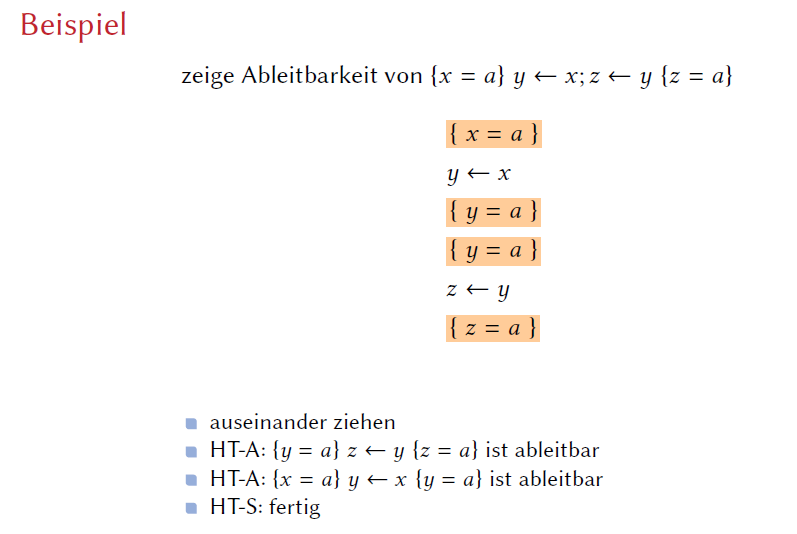
\includegraphics[scale=0.5]{hoare/bsp1}
\end{frame}

\begin{frame}{HT-I}
	\begin{minipage}{0.4\linewidth}
		\begin{align*}
			&\assert{ P } \\
			& \textbf{if } B \textbf{ then} \\
			&\hspace{2em} \assert{ P \wedge B } \\
			&\hspace{2em} S_1 \\
			&\hspace{2em} \assert{ Q }\\
			&\textbf{else} \\
			&\hspace{2em} \assert{ P \wedge \neg B } \\
			&\hspace{2em} S_2 \\
			&\hspace{2em} \assert{ Q }  \\
			&\textbf{fi}\\
			&\assert{Q }
		\end{align*}
	\end{minipage}
	\begin{minipage}{0.55\linewidth}
		\begin{block}{Regel HT-I \quad „If“}
			$\textbf{if } B\text{ } \textbf{ then } S_1 \textbf{ else } S_2 \textbf{ fi}$
			\smallskip
			\begin{itemize}
				\item Wenn $\{ P \wedge B \}\ S_1\ \{ Q \}$ gültig 
				\item und $\{ P \wedge \neg B \}\ S_2\ \{ Q \}$ gültig
				\item dann auch \\ $\{ P \} \textbf{ if } B \textbf{ then } S_1 \textbf{ else } S_2 \textbf{ fi } \{ Q \} $ gültig
			\end{itemize}
		\end{block}
%		\emph{HT4 : } $\textbf{if } B\text{ } \textbf{then } S_1 \textbf{ else } S_2 \textbf{ fi}$
%		\begin{itemize}
%			\item Wenn $\{ P \wedge B \} S_1 \{ Q \}$ gültig 
%			\item Wenn $\{ P \wedge \neg B \} S_2 \{ Q \}$ gültig
%			\item dann auch $\{ P \} \textbf{ if } B \textbf{ then } S_1 \textbf{ else } S_2 \textbf{ fi} \{ Q \} $ gültig
%		\end{itemize}
	\end{minipage}
\end{frame}

\begin{frame}{Beispiel: Berechnung von $\vert x \vert$}
	\vspace{-10mm}
	\begin{align*}
		&\assert{ x \in\R} \\
		&\textbf{if } x < 0 \textbf{ then } \\
		&\hspace{2em} \assert{ \visible<6->{ x\in\R\wedge x < 0 } } \\
		&\hspace{2em} \assert{ \visible<5->{ {-x} = \vert x \vert } } \\
		&\hspace{2em}  z \gets -x   \\
		&\hspace{2em} \assert{ \visible<2->{ z = \vert x \vert } } \\
		&\textbf{else} \\
		&\hspace{2em} \assert{ \visible<4->{ x\in\R\wedge x\geq 0 } } \\
		&\hspace{2em} \assert{ \visible<3->{ x = \vert x \vert } } \\
		&\hspace{2em} z \gets x \\
		&\hspace{2em} \assert{ \visible<2->{ z = \vert x \vert } } \\
		&\textbf{fi} \\
		&\assert{ z = \vert x \vert } 
	\end{align*}
\end{frame}

\begin{frame}{Aufgabe}
	\vspace{-10mm}
	  \begin{align*}
	&\assert{x=a \land y=b}  \\
	&\kw{if } x>y \kw{ then } \\
	&\hspace{2em} \assert{ \dots\ } \\
	&\hspace{2em}  z \gets y  \\
	&\hspace{2em} \assert{ \dots\ } \\
	&\kw{else } \\
	&\hspace{2em} \assert{ \dots\ } \\
	&\hspace{2em}  z \gets x  \\
	&\hspace{2em} \assert{ \dots\ } \\
	&\kw{fi } \\
	&\assert{z=\min(a,b)}
	\end{align*}
\end{frame}

\begin{frame}{Lösung}	
	\vspace{-2.5\baselineskip}
	\begin{alignat*}{2}
	&\assert{x=a \land y=b}  \\
	&\kw{if } x>y \kw{ then } \\
	&\hspace{2em} \assert{x=a \land y=b \land x>y} \\
	&\hspace{2em} \assert{y=\min(a,b)} \\
	&\hspace{2em}  z \gets y  \\
	&\hspace{2em} \assert{z=\min(a,b)} \\
	&\kw{else } \\
	&\hspace{2em} \assert{x=a \land y=b \land  \lnot (x>y)} \\
	&\hspace{2em} \assert{x=\min(a,b)} \\
	&\hspace{2em}  z \gets x  \\
	&\hspace{2em} \assert{z=\min(a,b)} \\
	&\kw{fi } \\
	&\assert{z=\min(a,b)}
	\end{alignat*}
\end{frame}


\mycomment{
%TODO: Lösung!!!
\begin{frame}{Jetzt seid ihr dran}
	\begin{align*}
	& z \gets x + y \\
	& z \gets z / 2 \\
	&\textbf{if } x \mod 2 = 0 \textbf{ then } \\
	&\hspace{2em} y \gets x + x \\
	&\hspace{2em} y \gets y / 4 \\
	&\textbf{else} \\
	&\hspace{2em} y \gets x - 1 \\
	&\hspace{2em} y \gets y / 2 \\
	&\textbf{fi} \\
	& z \gets z \· y \\
	&\assert{ z = div_2(a) \· (a+b)/2 } % WTF is div_2 ? => (2 `div`) ? a, b vs. x, y?
	\end{align*}
\end{frame}	
}


%\begin{frame}
%	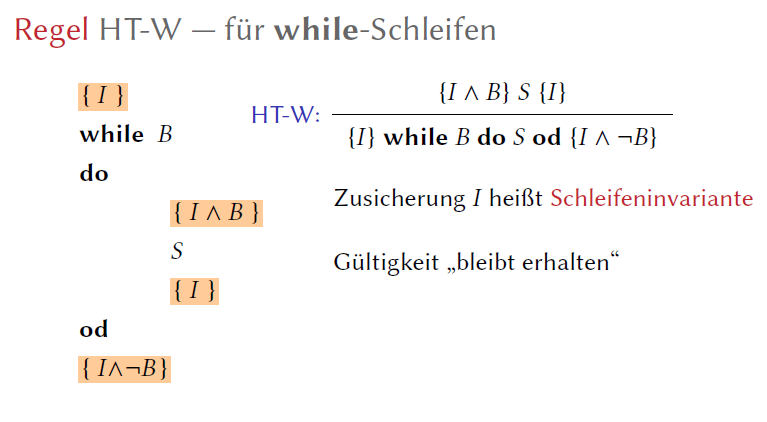
\includegraphics[scale=0.5]{hoare/htw}
%\end{frame}

\subsection{HT-W, Schleifeninvarianten}
\begin{frame}{HT-W}
	\begin{columns}[T] 
		\begin{column}[T]{.4\textwidth} 
			\vspace{-2\baselineskip}
			\begin{align*}
			&\assert{I} \q3uad \text{„Schleifeninvariante“} \\
			&\kw{while } B \kw{ do } \\
			&\qquad \assert{I \land B} \\
			&\qquad S \\
			&\qquad \assert{I} \\
			&\kw{od} \\
			&\assert{I \land \lnot B}
			\end{align*}
			\vspace{-1\baselineskip}
		\end{column}
		\begin{column}[T]{.4\textwidth} 
			\begin{block}{Regel HT-W \quad „While“}
				Wenn \htr{$I \land B$}{$S$}{$I$} gültig ist, dann ist auch die ganze \kw{while}-Schleife (s. links) gültig
			\end{block}
		\end{column}
	\end{columns}
	
	\pause
	\begin{block}{Schleifeninvarianten}
		\begin{itemize}
			\item sind Aussagen, die zu Beginn und Ende jedes Schleifendurchganges gültig sind
			\item helfen, die Korrektheit eines Programmes zu beweisen
			\item muss man ebenfalls beweisen 
			\item garantieren nicht die Korrektheit des Programms:\pause \\
			 Terminierung der Schleife muss zusätzlich gezeigt werden! (nicht in GBI)
		\end{itemize}
	\end{block}
\end{frame}
	
\begin{frame}{Beispiel Schleifeninvarianten}
	\begin{columns}
	\begin{column}[T]{0.49\linewidth}
	\begin{align*}
		&\assert{x=a \land y=b}  \\
		&\assert{ \dots\ } \\
		&\kw{while } y\not=0 \kw{ do } \\
		&\qquad\assert{ \dots } \\
		&\qquad y \gets y-1 \\
		&\qquad\assert{ \dots } \\
		&\qquad x \gets x+1 \\
		&\qquad\assert{ \dots\ } \\
		&\kw{od } \\
		&\assert{ \dots\ } \\ \pause
		&\assert{x=a+b} \\
	\end{align*}
	\end{column} 
	
	\begin{column}[T]{0.5\linewidth}
		\visible<2->{
			\bigskip
			\begin{block}{Wertetabelle für $a=3$ und $b=4$}
				\centering
				\medskip
				\begin{tabular}{c|cc}	 
					i & x & y \\ 
					\hline 
					0 & 3 & 4 \\
					1 & 4 & 3 \\
					2 & 5 & 2 \\
					3 & 6 & 1 \\
					4 & 7 & 0 \\
				\end{tabular}
			\end{block}
			\pause
			Schleifeninvariante: $$ x_i + y_i = a + b $$ 
		}
	\end{column}
	\end{columns}
\end{frame}

\begin{frame}{Beispiel Schleifeninvarianten}
	\vspace{-5mm}
	\begin{align*}
		&\assert{x=a \land y=b }  \\
		&\assert{ x+y=a+b }  \\
		&\kw{while } y\not=0 \kw{ do } \\
		&\qquad\assert{x+y=a+b \land y\not=0 }  \\
		&\qquad\assert{x+1+y-1=a+b } \\
		&\qquad y \gets y-1 \\
		&\qquad\assert{x+1+y = a+b} \\
		&\qquad x \gets x+1 \\
		&\qquad\assert{ x+y = a+b} \\
		&\kw{od } \\
		&\assert{ x+y = a+b \land (y=0) } \\
		&\assert{x=a+b} \\
	\end{align*}
\end{frame}

\begin{frame}{Exkurs: Schl.-Inv. mit Vollst. Induktion}
	Wir zeigen mit vollständiger Induktion die Gültigkeit der Schleifeninvariante. Dabei sei $i$ die Anzahl der bisher durchgelaufenen Schleifendurchläufe.\\
	
	\emph{Behauptung}: $$ \forall\ i \in \{0,...,b\} : x_i + y_i = a+b $$ \pause
	\begin{block}{Induktionsanfang}
		Für $i=0$ gilt $ x_0+y_0 = a+b $ nach Vorbedingung
	\end{block} \pause 
	\begin{block}{Induktionsvorrausetzung}
		Für ein beliebig aber festes $i\in \{0,...,b\}$ gelte die Behauptung
	\end{block}
\end{frame}

\begin{frame}{Exkurs: Schl.-Inv. mit Vollst. Induktion}
	\vspace{-2\baselineskip}
	\begin{align*}
	&\assert{x=a \land y=b}  \\
	&\assert{ x+y=a+b }\\
	&\kw{while } y\not=0 \kw{ do } \\
	&\qquad y \gets y-1 \\
	&\qquad x \gets x+1 \\
	&\kw{od } \\
	&\assert{x=a+b} \\
	\end{align*}
	\vspace{-2\baselineskip}
	\begin{block}{Induktionsschluss}
		Zu zeigen: $ x_{i+1} + y_{i+1} = a+b $ \pause
	%\vspace{-1.3\baselineskip}
		\begin{align*}
		x_{i+1}+y_{i+1} &= x_i +1 + y_i -1 \\
		&= x_i + y_i \\
		&\overset{IV}{=} a+b
		\end{align*}
	\end{block}
\end{frame}

\begin{frame} {Weitere Beispiele}
	Weitere Beispiele findet ihr hier: Übung 8, WS 15/16
\end{frame}

% TODO
% - Bäume (26)
% - Motivation - das kann man noch deutlich besser machen. (Aber wie?)
% - evtl. Strenger Zusammenhang


\section{Graphen}

\begin{frame}{Ein Graph}
	
	\begin{figure}[H]
		\begin{tikzpicture}[->,>=stealth,baseline=-5mm]
		\matrix[matrix of math nodes,nodes={draw,circle,minimum size=10mm,inner sep=2pt},row sep=15mm,column sep=15mm,ampersand replacement=\&]
		{
			|(1)| 1 \& |(3)| 3 \\
			|(0)| 0 \& |(2)| 2  \\
		};
		\draw  (0) -- (1);
		\draw  (1) -- (2);
		\draw  (2) -- (3);
		\draw  (3) -- (1);
		
		\end{tikzpicture}
	\end{figure}
	
\end{frame}

\begin{frame}{Graphen -- Wofür?}
	\begin{itemize}
		\item Straßennetze und andere Verkehrsnetze (Kürzeste Wege)
		\item Kabelnetze (Minimale Spannbäume)
		\item Rohrnetze (Maximaler Fluss)
	\end{itemize}

	\begin{block}{Zitat}
		\enquote{Egal für wie wichtig du Graphen in der Informatik hältst, sie sind mindestens doppelt so wichtig!}\\
		\emph{Ein Google-Manager über Einstellungsgespräche bei Google}
	\end{block}
\end{frame}

\subsection{Definitionen}

\begin{frame}{Graphen}
	\begin{Definition}
		Ein \textbf{gerichteter Graph} ist ein Paar $G = (V, E)$ mit einer \emph{endlichen}, \emph{nichtleeren} Menge an \textbf{Knoten} $V$ und einer Menge an \textbf{Kanten}\\
		$E \subseteq V \times V$.
	\end{Definition} \pause
	$E$ enthält also Paare (geordnet) von Elementen aus $V$. \pause
	
	\bigskip
	\begin{Definition}
		Ein \textbf{ungerichteter Graph} ist ein Paar $G = (V, E)$ mit einer \emph{endlichen}, \emph{nichtleeren} Menge an \textbf{Knoten} $V$ und einer Menge an \textbf{Kanten}\\
		$E \subseteq \set{ \{x,y\} \Mid x \in V \land y \in V }$.
	\end{Definition} \pause
	$E$ enthält also Mengen (ungeordnet) mit je ein oder zwei Elementen aus $V$!
\end{frame}

\begin{frame}{Graphen}
	\begin{block}{Hinweis}
		Häufig wählt man $V = \Z_k = \{0,1,2,...,k-1\}$\\
		
		Da $V$ immer endlich ist, muss auch $E$ endlich sein.\\
		$E = \emptyset$ geht aber!
	\end{block}

	\pause
	\begin{Definition}
		Zwei Knoten $x$ und $y$ in einem Graphen $G$ heißen \textbf{adjazent}, wenn eine Kante von $x$ nach $y$ zeigt.
	\end{Definition}
	\textbf{Achtung}: Im gerichteten Fall ist diese Aussage nicht symmetrisch!

	\pause
	\begin{Definition}
		Eine Kante mit identischem Start- und Endpunkt nennt man \textbf{Schlinge}.\\
		Also $(x,x) \in E$ (gerichtet) bzw. $\{x\} \in E$ (ungerichtet).\\
	\end{Definition}
\end{frame}

\begin{frame}{Beispiel}
	Wir betrachten den gerichteten Graphen $G = (V, E)$ mit $V = \{0,1,2,3,4,5\}$ und $E = \set{(0,1), (1,0), (1,2), (3,4), (4,3) ,(4,5)}$
	\bigskip

	\begin{figure}[H]
		\begin{tikzpicture}[->,>=stealth,baseline=-5mm]
		\matrix[matrix of math nodes,nodes={draw,circle,minimum size=10mm,inner sep=2pt},row sep=15mm,column sep=15mm,ampersand replacement=\&]
		{
			|(1)| 1 \& |(5)| 5 \& |(3)| 3 \\
			|(0)| 0 \& |(2)| 2 \& |(4)| 4 \\
		};
		\draw  (0) to [bend left] (1);
		\draw  (1) to [bend left] (0);
		\draw  (1) -- (2);
		
		\draw  (4) -- (5);
		\draw  (4) to [bend left] (3);
		\draw  (3) to [bend left] (4);
		\end{tikzpicture}
	\end{figure}

\end{frame}

\begin{frame}{Aufgabe: Graphen zeichnen}
	Zeichnet die Graphen $G_i = (V, E_i)$ mit $V = \Z_4$ und
	$E_1 = \set{(0,1), (0,2), (0,3), (1,2), (1,3), (2,2), (2,3), (3,2)}$\\
	$E_2 = \set{\{0,1\}, \{0,2\}, \{0,3\} }$\\
	$E_3 = \emptyset$\\
	$E_4 = V \times V$\\
	$E_5 = \set{(0,1), (1,2), (1,3)}$
\end{frame}

\begin{frame}[t]{Lösung: Graphen zeichnen}
	Zeichnet den Graphen $G_1 = (V, E_1)$ mit
	$$V = \Z_4 \qquad E_1 = \{(0,1), (0,2), (0,3), (1,2), (1,3), (2,2), (2,3), (3,2)\}$$
	
	\pause
	\bigskip
	\begin{figure}[H]
		\begin{tikzpicture}[->,>=stealth,baseline=-5mm]
			\matrix[matrix of math nodes,nodes={draw,circle,minimum size=10mm,inner sep=2pt},row sep=15mm,column sep=15mm,ampersand replacement=\&]
			{
				|(0)| 0 \& |(1)| 1 \& |(2)| 2 \\
				\& |(3)| 3 \& \\
			};
			\draw  (0) -- (1);
			\draw  (0) -- (3);
			\draw  (2)  to [bend left] (3);
			\draw  (1) -- (2);
			\draw  (3) to [bend left] (2);
			\draw  (0) to [bend left]  (2);
			\path (2) edge [loop right] ();
			\draw (1) -- (3);
		\end{tikzpicture}
	\end{figure}
\end{frame}

\begin{frame}[t]{Lösung: Graphen zeichnen}
	Zeichnet den Graphen $G_2 = (V, E_2)$ mit
	$$V = \Z_4 \qquad E_2 = \{\{0,1\}, \{0,2\}, \{0,3\} \}$$
	
	\pause
	\bigskip
	\begin{figure}[H]
		\begin{tikzpicture}[-,>=stealth,baseline=-5mm]
		\matrix[matrix of math nodes,nodes={draw,circle,minimum size=10mm,inner sep=2pt},row sep=15mm,column sep=15mm,ampersand replacement=\&]
		{
			|(0)| 0 \& |(1)| 1 \& |(2)| 2 \\
			\& |(3)| 3 \& \\
		};
		\draw  (0) -- (1);
		\draw  (0)  to [bend left] (2);
		\draw  (0) -- (3);
		\end{tikzpicture}
	\end{figure}
\end{frame}

\begin{frame}[t]{Lösung: Graphen zeichnen}
	Zeichnet den Graphen $G_3 = (V, E_3)$ mit
	$$V = \Z_4 \qquad E_3 = \emptyset$$
	
	\pause
	\bigskip
	\begin{figure}[H]
		\begin{tikzpicture}[->,>=stealth,baseline=-5mm]
		\matrix[matrix of math nodes,nodes={draw,circle,minimum size=10mm,inner sep=2pt},row sep=15mm,column sep=15mm,ampersand replacement=\&]
		{
			|(0)| 0 \& |(1)| 1 \& |(2)| 2 \\
			\& |(3)| 3 \& \\
		};
		\end{tikzpicture}
	\end{figure}
\end{frame}

\def\bend{8}
\begin{frame}[t]{Lösung: Graphen zeichnen}
	Zeichnet den Graphen $G_4 = (V, E_4)$ mit
	$$V = \Z_4 \qquad E_4 = V \times V$$
	
	\pause
	\bigskip  %TODO!!
	\begin{figure}[H]
		\begin{tikzpicture}[->,>=stealth,baseline=-5mm]
		\matrix[matrix of math nodes,nodes={draw,circle,minimum size=10mm,inner sep=2pt},row sep=25mm,column sep=25mm,ampersand replacement=\&]
		{
			|(0)| 0 \& |(1)| 1 \\
			|(2)| 2 \& |(3)| 3 \\
		};
		\path (0) edge [loop left] ();
		\path (1) edge [loop right] ();
		\path (2) edge [loop left] ();
		\path (3) edge [loop right] ();
		
		\draw  (0) to [bend left=\bend] (1);
		\draw  (0) to [bend left=\bend] (2);
		\draw  (0) to [bend left=\bend] (3);
		\draw  (1) to [bend left=\bend] (0);
		\draw  (1) to [bend left=\bend] (2);
		\draw  (1) to [bend left=\bend] (3);
		\draw  (2) to [bend left=\bend] (0);
		\draw  (2) to [bend left=\bend] (1);
		\draw  (2) to [bend left=\bend] (3);
		\draw  (3) to [bend left=\bend] (0);
		\draw  (3) to [bend left=\bend] (1);
		\draw  (3) to [bend left=\bend] (2);
		
		
		\end{tikzpicture}
	\end{figure}
\end{frame}

\begin{frame}[t]{Lösung: Graphen zeichnen}
	Zeichnet den Graphen $G_5 = (V, E_5)$ mit
	$$V = \Z_4 \qquad E_5 = \{ (0,1), (1,2), (1,3) \}$$
	
	\pause
	\bigskip
	\begin{figure}[H]
		\begin{tikzpicture}[->,>=stealth,baseline=-5mm]
		\matrix[matrix of math nodes,nodes={draw,circle,minimum size=10mm,inner sep=2pt},row sep=15mm,column sep=15mm,ampersand replacement=\&]
		{
			|(0)| 0 \& |(1)| 1 \& |(2)| 2 \\
			\& |(3)| 3 \& \\
		};
		\draw  (0) -- (1);
		\draw  (1) -- (2);
		\draw  (1) -- (3);
		\end{tikzpicture}
	\end{figure}
\end{frame}



\begin{frame}{Teilgraphen}
	\begin{Definition}
		Ein \textbf{Teilgraph} $T = (V',E')$ von $G$ ist ein Graph, den man kriegt, wenn man aus $G$ beliebige Knoten und Kanten so wegwirft, dass keine Kante \enquote{in die Luft} zeigt.  Also (für gerichtete Graphen):
		%Ein \textbf{Teilgraph} $T = (V',E')$ von $G$ ist ein Graph, bei dem Knoten- und Kantenmenge Teilmengen des Graphens $G$ sind und deren Kanten nicht aus dem Teilgraph hinausführen. Also (für gerichtete Graphen):
		$$V' \subseteq V \qquad E' \subseteq E \cap (V' \times V')$$
	\end{Definition} \pause

	Hinweis: Natürlich dürfen wir in $E'$ auch Kanten aus $E \cap (V' \times V')$ \enquote{weglassen}!
\end{frame}

\begin{frame}{Teilgraphen: Beispiel}
	\begin{columns}
		\column[T]{0.3 \linewidth}
		
		\begin{tikzpicture}[->,>=stealth,baseline=-5mm]
		\matrix[matrix of math nodes,nodes={draw,circle,minimum size=5mm,inner sep=2pt},row sep=10mm,column sep=10mm,ampersand replacement=\&]
		{
			|(0)| 0 \& |(1)| 1 \& |(2)| 2 \\
			\& |(3)| 3 \& \\
		};
		\draw  (0) -- (1);
		\draw  (0) -- (3);
		\draw  (2)  to [bend left] (3);
		\draw  (1) -- (2);
		\draw  (3) to [bend left] (2);
		\draw  (0) to [bend left]  (2);
		\path (2) edge [loop right] ();
		\draw (1) -- (3);
		\end{tikzpicture}
		\begin{center}
			Graph $G$
		\end{center}
		
		\pause
		\column[T]{0.3 \linewidth}
		\begin{tikzpicture}[->,>=stealth,baseline=-5mm]
		\matrix[matrix of math nodes,nodes={draw,circle,minimum size=5mm,inner sep=2pt},row sep=10mm,column sep=10mm,ampersand replacement=\&]
		{
			|(0)| 0 \& |(1)| 1 \& |(2)| 2 \\
			\&  \& \\
		};
		\draw  (0) -- (1);
		\draw  (1) -- (2);
		\draw  (0) to [bend left]  (2);
		\end{tikzpicture}
		\begin{center}
			Teilgraph $T_1$ von $G$
		\end{center}
		
		\pause
		\column[T]{0.3 \linewidth}
		\begin{tikzpicture}[->,>=stealth,baseline=-5mm]
		\matrix[matrix of math nodes,nodes={draw,circle,minimum size=5mm,inner sep=2pt},row sep=10mm,column sep=10mm,ampersand replacement=\&]
		{
			|(0)| 0 \& |(1)| 1 \& |(2)[white]| 2 \\  % (2): stealth node
			        \& |(3)| 3 \& \\
		};
		\draw[->, white]  (0) to [bend left] (2); % stealth edge
		\draw  (0) -- (1);
		\draw  (0) -- (3);
		\draw (1) -- (3);
		\end{tikzpicture} 
		\begin{center}
			Teilgraph $T_2$ von $G$
		\end{center}
	\end{columns}
\end{frame}

\begin{frame}{Teilgraphen: Beispiel}
	\begin{columns}
		\column[T]{0.3 \linewidth}
		
		\begin{tikzpicture}[->,>=stealth,baseline=-5mm]
		\matrix[matrix of math nodes,nodes={draw,circle,minimum size=5mm,inner sep=2pt},row sep=10mm,column sep=10mm,ampersand replacement=\&]
		{
			|(0)| 0 \& |(1)| 1 \& |(2)| 2 \\
			\& |(3)| 3 \& \\
		};
		\draw  (0) -- (1);
		\draw  (0) -- (3);
		\draw  (2)  to [bend left] (3);
		\draw  (1) -- (2);
		\draw  (3) to [bend left] (2);
		\draw  (0) to [bend left]  (2);
		\path (2) edge [loop right] ();
		\draw (1) -- (3);
		\end{tikzpicture}
		\begin{center}
			Graph $G$
		\end{center}
		
		\column[T]{0.5 \linewidth}
		\begin{tikzpicture}[->,>=stealth,baseline=-5mm]
		\matrix[matrix of math nodes,nodes={draw,circle,minimum size=5mm,inner sep=2pt},row sep=10mm,column sep=10mm,ampersand replacement=\&]
		{
			|(2)[white]| 2  \& |(0)| 0 \& |(1)[white]| 1 \\ % (1), (2): stealth nodes
			\& \& |(3)[white]| 3  \\
		};
		\draw[myalertcolor]  (0) -- (1);
		\draw[myalertcolor]  (0) -- (3);
		\draw[->, white]  (2) to [bend left] (1); % stealth edge
		\end{tikzpicture}
		\begin{center}
			...ist überhaupt kein Graph \\ \impl auch kein Teilgraph!
		\end{center}
	\end{columns}	
\end{frame}

\begin{frame}{Knotengrade}
	
	\begin{Definition}
		In \emph{gerichteten} Graphen:
		Der \textbf{Eingangsgrad} eines Knoten $k$ ist die Anzahl der Knoten, die auf $k$ zeigen. \\
		Der \textbf{Ausgangsgrad} eines Knoten $k$ ist die Anzahl der Knoten, die von $k$ wegzeigen.  Also: 
		\begin{align*}
			d^-(k) = \abs{\set{ x \Mid (x,k) \in E}} \\
			d^+(k) = \abs{\set{ x \Mid (k,x) \in E}}
		\end{align*}
		\pause
		Der \textbf{Grad} eines Knotens $k$ ist $d(k) = d^+(k) + d^-(k)$.
	\end{Definition}

	\pause
	\bigskip
	In \emph{ungerichteten} Graphen (bei uns!):\\
	Knotengrad $d(k)$ ist Anzahl der \enquote{Linien}, die $k$ berühren.\\
	Schlingen zählen also zweifach!
	%Also tatsächlich \enquote{Anzahl der Berührungen von Linien mit dem Kreis}.
\end{frame}

\subsection{Pfade und Wege}
\begin{frame}{Pfade und Wege}
	\begin{Definition}
		Sei $G$ ein \emph{gerichteter / ungerichteter} Graph.\\
		Ein \textbf{Pfad / Weg} ist eine Folge von Knoten, die jeweils über Kanten im Graphen erreichbar sind. Also eine \alert{nichtleere} Liste $$p = (v_0, v_1, \dots, v_n) \quad \text{mit} \quad (v_i, v_{i+1}) \in E$$
	\end{Definition}
	\pause
	Die Länge eines Pfades ist die Anzahl der Kanten \quad $n = \abs{p} - 1$ \; (!). \\
	\smallskip
	$w$ heißt \textbf{von $v$ erreichbar}, wenn es einen Pfad von $v$ nach $w$ gibt.
	\begin{Beispiel}
		Sei $G = (V, E)$ mit $V = \Z_9, \quad E = V \times V$\\ \pause
		$p_1 = (7)$ ist ein Pfad der Länge 0.\\
		$p_2 = (0, 1, 2, 3, 0)$ ist ein Pfad der Länge 4.
	\end{Beispiel}
\end{frame}

\begin{frame}[t]{Pfade}
	Sei $G$ ein gerichteter Graph. Ein Pfad $p = (v_0, \dots, v_n)$ heißt
	\begin{tabular}{>{\itshape}rp{.7\textwidth}}
		geschlossen & wenn $v_0 = v_n$ gilt  \\
		Zyklus & wenn er geschlossen ist und Länge $\geq 1$ gilt \\
		wiederholungsfrei & Wenn alle Knoten paarweise verschieden sind \newline ($v_0 = v_n$ geht aber!) \\
		einfacher Zyklus &  wenn er ein wiederholungsfreier Zyklus ist  \\
	\end{tabular}
	\medskip \\
	\textbf{Azyklischer} Graph: Graph ohne Zyklen\\
	\impl Oftmals auch DAG (Directed Acyclic Graph)
\end{frame}

\begin{frame}[t]{Wege}
	Sei $G$ ein \alert{un}gerichteter Graph. Ein \alert{Weg} $p = (v_0, \dots, v_n)$ heißt
	\begin{tabular}{>{\itshape}rp{.7\textwidth}}
		geschlossen & wenn $v_0 = v_n$ gilt  \\
		\alert{Kreis} & wenn er geschlossen ist und Länge $\geq 1$ gilt \\
		wiederholungsfrei & Wenn alle Knoten paarweise verschieden sind \newline ($v_0 = v_n$ geht aber!) \\
		einfacher \alert{Kreis} &  wenn er ein wiederholungsfreier Kreis \alert{mit mind. 3~versch. Knoten} ist  \\
	\end{tabular}

\end{frame}

\begin{frame}{Teilpfade}
	\begin{Definition}
		Ein \emph{Teilpfad} eines Pfades entsteht durch Streichen von Knoten am Anfang und/oder Ende des Pfades.
	\end{Definition}

	\pause
	\begin{block}{Beachte}
		Mindestens einen Knoten übrig lassen! (Sonst kein gültiger Pfad mehr)\\
		Es darf \textbf{nicht} aus der Mitte gestrichen werden! (Sonst evtl. kein Pfad mehr, wenn die entsprechenden Kanten nicht im Graphen vorhanden sind)
	\end{block}

	\pause
	\begin{Beispiel}
		Sei $p = (1, 2, 3, 4, 5, 1)$ und $G$ passend gewählt.\\
		\pause
		$(2, 3), (1, 2, 3, 4, 5), (4, 5, 1)$ sind Teilpfade\\
		$(), (1, 2, 1), (1, 2, 3, 4, 5, 1, 2)$ sind keine Teilpfade.
	\end{Beispiel}
\end{frame}

%TODO Beispiel Pfade
%Beispiel machen, in dem zwar ein Pfad von x nach y existiert, aber nicht umgekehrt.
%• beachte: für aufeinanderfolgende Knoten im Pfad muss die Kante in die richtige Richtung
%weisen!
%• Beachte: Knoten dürfen in Pfad mehrfach vorkommen
%• Beispiel machen, in dem von x nach y unterschiedlich lange Pfade vorkommen

\begin{frame}{Gerichtet $\leftrightsquigarrow$ ungerichtet umwandeln}
	Einen gerichteten Graphen $G = (V,E)$ kann man in den \textbf{zu $G$ gehörigen ungerichteten Graphen} umwandeln, indem man die Pfeilspitzen weglässt. \\
	
	\medskip
	Andersrum: Aus einer Kante zwei machen und Pfeile in beide Richtungen.
	
	%TODO (strenger) Zusammenhang
	%\bigskip
	%$G$ gerichtet heißt \textbf{streng zusammenhängend}.....
\end{frame}

\begin{frame}{Gerichtete Bäume}
	\begin{Definition}
		Ein gerichteter Graph $T$ heißt \textbf{Baum} \Gdw Es gibt eine \textbf{Wurzel} $r \in V$, sodass zu jedem Knoten \emph{genau ein Pfad} von $r$ aus existiert. \\
		\smallskip
		Diese Wurzel ist eindeutig und hat Eingangsgrad $= 0$. \\
		\textbf{Blätter} sind Knoten mit Ausgangsgrad $= 0$. \\
		\textbf{Innere Knoten} sind Knoten mit Ausgangsgrad $> 0$. 
		
	\end{Definition}
\end{frame}

\begin{frame}{Ungerichtete Bäume}
	\begin{Definition}
		Ein ungerichteter Graph $T$ heißt \textbf{Baum} \Gdw Es gibt einen gerichteten Baum, den man zum ungerichteten $T$ umwandeln kann. \\
		\smallskip
		Dessen Wurzel ist \textbf{nicht} eindeutig.
		
	\end{Definition}
\end{frame}

\begin{frame}{Isomorphie}
	Zwei Graphen heißen \textbf{isomorph}, wenn sie \enquote{bis auf eine Umbenennung der Knoten identisch sind}, also die gleiche Struktur besitzen.\\
	
	\pause
	\medskip
	
	Formal: Haben $G_1 = (V_1, E_1), \, G_2 = (V_2, E_2)$. \\
	$G_1$ \textbf{isomorph} zu $G_2$, wenn es eine Bijektion $f \from V_1 \functionto V_2$ gibt mit \[\forall x,y \in V_1: \quad (x,y) \in E_1 \gdw \tuple{f(x),f(y)} \in E_2. \]
	
	$f$ heißt dann auch \emph{(Graph-)Isomorphismus}.
	
\end{frame}

\begin{frame}{Aufgabe Graphisomorphie}
	\begin{block}{Aufgabe (WS 2010)}
		Jeweils zwei der sechs Graphen sind isomorph zueinander. Geben Sie die Paare von isomorphen Graphen sowie den zugehörigen Isomorphismus ($=$~„Umbenennung“) in Tabellenform an.
		\begin{figure}[H]
			\centering
			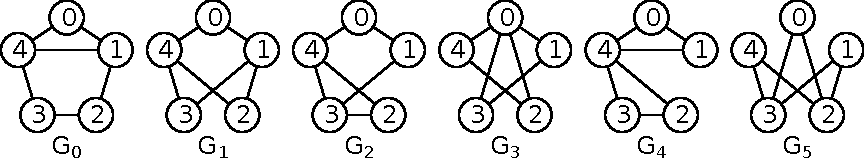
\includegraphics[scale=0.7]{Graphen/Graph_Iso.pdf}
		\end{figure}
	\end{block}
	Tipp: Nach \enquote{markanten} Knoten (Knoten mit hohem Grad) suchen.\\
	Oftmals hierdurch bereits Ausschluss möglich.
\end{frame}

\begin{frame}{Lösung}
	\begin{figure}[H]
		\centering
		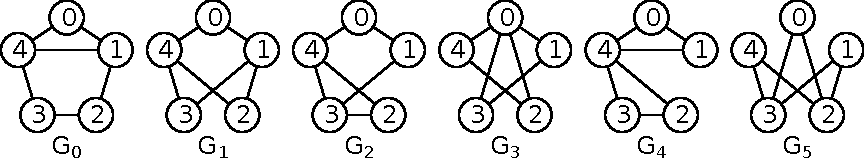
\includegraphics[scale=0.7]{Graphen/Graph_Iso.pdf}
	\end{figure}
	\begin{table}[H]
		\centering
		\begin{tabular}{c|c|c|c|c|c}
			$G_0: $ & 0 & 1 & 2 & 3 & 4 \\
			$G_2: $ & 2 & 3 & 1 & 0 & 4 \\[1em]
			$G_3: $ & 0 & 1 & 2 & 3 & 4 \\
			$G_4: $ & 4 & 0 & 2 & 1 & 3 \\[1em]
			$G_1: $ & 0 & 1 & 2 & 3 & 4 \\
			$G_5: $ & 0 & 2 & 1 & 4 & 3 \\
		\end{tabular}
	\end{table}
\end{frame}

% TODO: Ändern zu Abschnitt über Äquivalenzrelationen in Graphen
%Falls schon Fragen kommen: mit dem Bild einer Nicht-Äquivalenzrelation anfangen und
%so lange Pfeile dazu malen, bis alle Forderungen erfüllt sind:
%• Schlingen an allen Knoten
%• zu jedem Pfeil hin auch der zurück
%• wenn ein Pfad von x nach y existiert, dann auch eine direkte Kante
%Ergebnis: einige Klumpen, äh, Cliquen (die den Äquivalenzklassen entsprechen)

%Pfade, E^*
%• E2 ist wieder Relation auf V: kann man also als Graph malen: Beispiel machen
%• analog für E3, . . .
%• und E^* ist auch wieder eine Relation auf V: kann man also als Graph malen: Beispiel:
%aus Zyklus der Länge 5 wird der sogenannte vollständige Graph K5

%\subsection{Graphen und Relationen}
%\begin{frame}
%	\frametitle{Graphen und Relationen}
%	Wenn $G=(V,E)$ ein (un)gerichteter Graph ist, dann ist $E$ eine binäre Relation. \\ \vspace{2em} \pause
%	Wann ist sie symmetrisch, transitiv, reflexiv? Bzw. was bedeutet das? \\ \vspace{2em} \pause 
%	Was ist $E^i$? Was ist $E^\ast$? Was heißt $E^\ast = V \times V$? 
%\end{frame}

%% Übungsaufgaben
\section{Aufgaben}

\begin{frame}{Maximale Kanten}
	Sei $G$ ein \textbf{gerichteter} Graph mit $n$ Knoten. Wie viele Kanten kann $G$ maximal haben... \\[0.2in]
	
	Wenn Schlingen erlaubt sind? \pause \\ 
	$n^2$  \\[0.3in]
	
	Wenn er schlingenfrei ist? \pause\\ 
	$n^2 - n = n \· (n-1)$		
\end{frame}

\begin{frame}{Maximale Kanten}
	Sei $G$ ein \textbf{ungerichteter} Graph mit $n$ Knoten. Wie viele Kanten kann $G$ maximal haben... \\[0.2in]
	
	\visible<3->{Wenn Schlingen erlaubt sind? \\ }
	\visible<4->{$\frac{n(n+1)}{2} \qquad \left( = \frac{n(n-1)}{2} + n\right)$ \\[0.3in]}
	
	Wenn er schlingenfrei ist? \\
	\visible<2->{$\frac{n(n-1)}{2} $\\ Man verbindet jeden Knoten mit den jeweils anderen Knoten, fasst dann jeweils 2 gleiche Kanten zusammen.}
\end{frame}

\begin{frame}{Aufgabe (WS 2008) \stars{2}}
	\begin{itemize}	
		\item Zeichnen Sie alle möglichen gerichteten Bäume mit genau vier Knoten, von denen keine zwei isomorph sind.
		\item Zeichnen Sie alle möglichen ungerichteten Bäume mit genau fünf Knoten, von denen keine zwei isomorph sind.
	\end{itemize}
\end{frame}

\begin{frame}{Lösung}
	\textit{Zeichnen Sie alle möglichen gerichteten Bäume mit genau vier Knoten, von denen keine zwei isomorph sind.} \pause
	\begin{center}
		\begin{minipage}{0.3\linewidth}
			\vspace*{\fill}
			\centering
			
\includegraphics[scale=0.2]{Graphen/baume1.pdf} 
			\vfill
		\end{minipage}
		\begin{minipage}{0.2\linewidth}
			\vspace*{\fill}
			\centering
			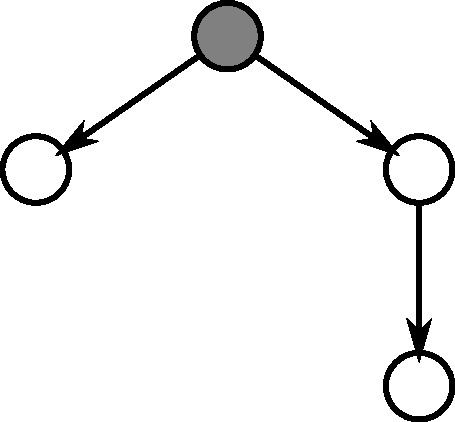
\includegraphics[scale=0.2]{Graphen/baume2.pdf} 
			\vfill
		\end{minipage}
		\begin{minipage}{0.2\linewidth}
			\vspace*{\fill}
			\centering
			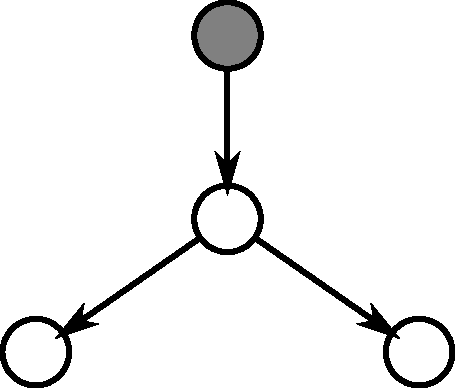
\includegraphics[scale=0.2]{Graphen/baume3.pdf} 
			\vfill
		\end{minipage}
		\begin{minipage}{0.2\linewidth}
			\vspace*{\fill}
			\centering
			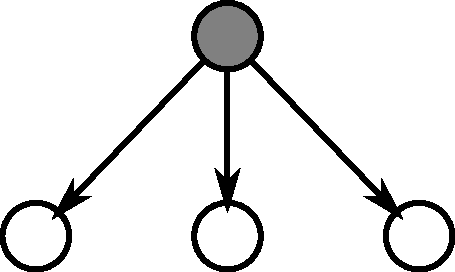
\includegraphics[scale=0.2]{Graphen/baume4.pdf} 
			\vfill
		\end{minipage}
	\end{center} \pause
	\textit{Zeichnen Sie alle möglichen ungerichteten Bäume mit genau fünf Knoten, von denen keine zwei isomorph sind.} \pause
	\begin{center}
		\begin{minipage}{0.2\linewidth}
			\vspace*{\fill}
			\centering
			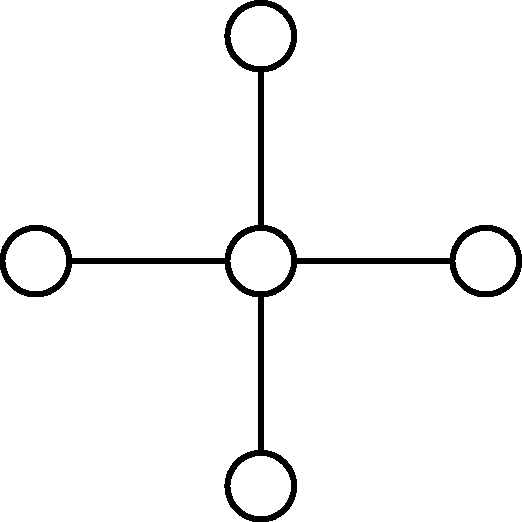
\includegraphics[scale=0.2]{Graphen/baume5.pdf} 
			\vfill
		\end{minipage}
		\begin{minipage}{0.25\linewidth}
			\vspace*{\fill}
			\centering
			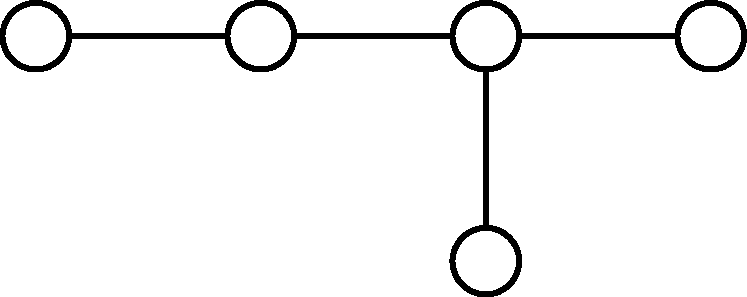
\includegraphics[scale=0.2]{Graphen/baume6.pdf} 
			\vfill
		\end{minipage}
		\begin{minipage}{0.35\linewidth}
			\vspace*{\fill}
			\centering
			
\includegraphics[scale=0.2]{Graphen/baume7.pdf} 
			\vfill
		\end{minipage}
	\end{center}
\end{frame}


\begin{frame}{Aufgabe: Bäume (WS 2010) \stars{1}}
	Sei $T_1 = (V_1 , E_1 )$ ein gerichteter Baum mit Wurzel $r_1$, $T_2 = (V_2 , E_2 )$ ein gerichteter Baum mit Wurzel $r_2$, und es gelte $V_1 \cap V_2 = \{\}$. Sei $r \not\in V_1 \cup V_2$. \\
Zeigen Sie: $$T_1 \circ_r T_2 = (V_1 \cup V_2 \cup {r}, E_1 \cup E_2 \cup \{(r, r_1 ), (r, r_2 )\})$$ ist ein gerichteter Baum mit Wurzel $r$.
\end{frame}

\begin{frame}{Lösung}
	\textit{Zeigen Sie: $$T_1 \circ_r T_2 = (V_1 \cup V_2 \cup {r}, E_1 \cup E_2 \cup \{(r, r_1 ), (r, r_2 )\})$$ ist ein gerichteter Baum mit Wurzel $r$.} \\[2em] \pause
	Zwei Dinge sind zu zeigen:
	\begin{itemize}[<+->]
		\item Zu jedem $v \in V_1 \cup V_2 \cup {r}$ gibt es einen Pfad von $r$ aus
		\item Dieser Pfad ist eindeutig.
	\end{itemize}
\end{frame}

\begin{frame}{Lösung}
	\textit{Wir zeigen zuerst, dass es von $r$ zu jedem Knoten $v \in V_1 \cup V_2 \cup \{r\}$ einen Pfad
gibt.} \\[2em]
	\pause
	\begin{itemize}[<+->]
		\item Es gibt offensichtlich einen Pfad (der Länge 0) von $r$ nach $r$.
		\item Sei $v \in V_1$. Dann gibt es nach Definition einen Pfad von $r_1$ nach $v$ über den Baum $T_1$ und dessen Kanten $E_1$. Da in $T_1 \circ_r T_2$ auch der Pfad $r$ nach $r_1$ liegt, gibt es also einen Pfad von $r$ nach $v$ in $T_1 \circ_r T_2$.
		\item Analog zu $v \in V_2$.
	\end{itemize}
	\visible<5>{Somit gibt es für alle Knoten $v \in V_1 \cup V_2 \cup \{r\}$ einen Pfad von $r$ nach $v$.}
\end{frame}

\begin{frame}{Lösung}
	\textit{Wir zeigen nun noch, dass es für keinen Knoten zwei verschiedenen Pfade von r nach v gibt.} \\[2em]\pause
	Für $v = r$ gibt es offensichtlich keine zwei verschiedenen Pfade. \pause \\ Sei also exemplarisch $v \in V_1$. Da $V_1 \cap V_2 = \{\}$, sind von $r_2$ nur Elemente aus $V_2$ zu erreichen. Somit muss ein Pfad von $r$ nach $v$ über $r_1$ gehen (weil von $r_2$ kein Pfad zurück führt). \pause Da $T_1$ aber ein Baum ist, ist der Pfad von $r_1$ nach $v$ eindeutig. Der Pfad von $r$ nach $r_1$ ebenso. \pause Also ist der Pfad von $r$ nach $v$ auch eindeutig. Analog zu $v \in V_2$.
\end{frame}

% Pufferaufgabe
\begin{frame}{Aufgabe (WS 2009) \stars{4}}
	Eine Zahl $n$ ist genau dann eine Primzahl, wenn sie eine positive ganze Zahl ist und genau zwei Teiler hat, nämlich 1 und n. Insbesondere ist 1 keine Primzahl. \\
	Für $n \in \N^+$ sei der Graph $G_n = (V_n , E_n )$ gegeben durch
	$$V_n =\set{m \in \N^+ \Mid m \text{ teilt } n} \quad \text{und}$$
	$$E_n =\set{(k, m) \in V_n \times V_n \Mid k \text{ teilt } m \text{ und } m/k  \text{ ist eine Primzahl}}.$$
	\begin{itemize}
		\item Zeichnen Sie $G_{12}$ , $G_{16}$ und $G_{30}$.
		\item Zeigen Sie: $$\forall n, m \in \N^+: n \text{ teilt } m \impl G_n \text{ ist Teilgraph von } G_m.$$
	\end{itemize}
\end{frame}

\begin{frame}{Lösung}
	$$V_n =\set{m \in \N^+ \Mid m \text{ teilt } n}, $$
	$$E_n =\set{(k, m) \in V_n \times V_n \Mid k \text{ teilt } m \text{ und } m/k  \text{ ist eine Primzahl}}.$$
	\textit{Zeichnen Sie $G_{12}$ , $G_{16}$ und $G_{30}$.} \\[1,5em]
	
	\visible<2>{
		\begin{center}
			\begin{minipage}{0.2\linewidth}
				\vspace*{\fill}
				\centering
				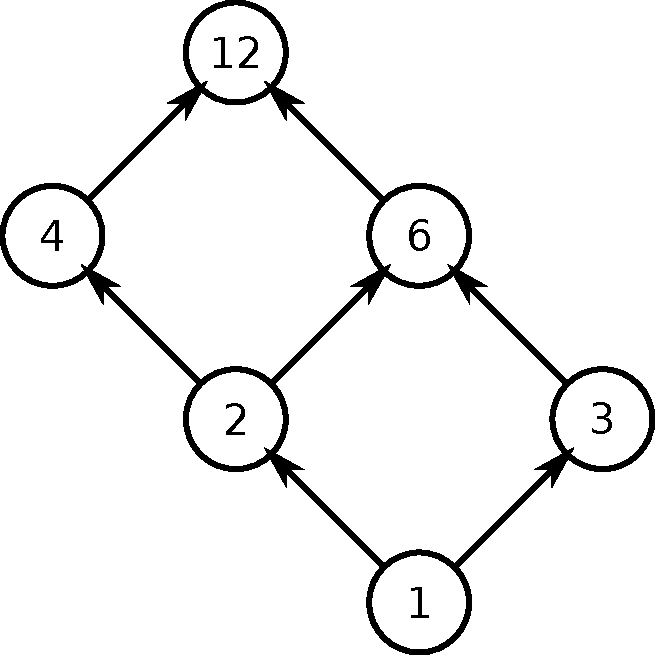
\includegraphics[scale=0.2]{Graphen/Primzahlen1.pdf} 
				\vfill
			\end{minipage}
			\begin{minipage}{0.5\linewidth}
				\vspace*{\fill}
				\centering
				
\includegraphics[scale=0.2]{Graphen/Primzahlen2.pdf} 
				\vfill
			\end{minipage}
			\begin{minipage}{0.2\linewidth}
				\vspace*{\fill}
				\centering
				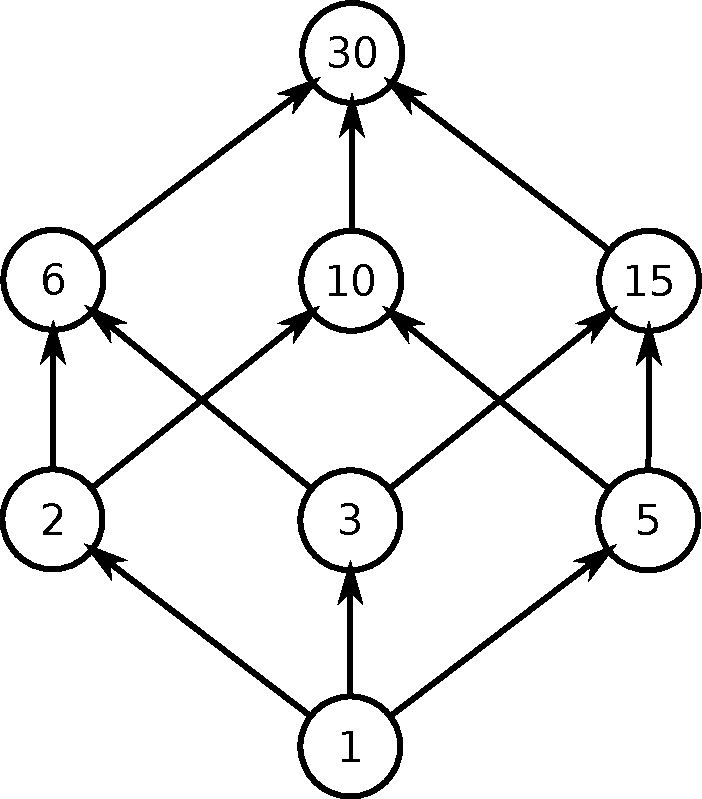
\includegraphics[scale=0.2]{Graphen/Primzahlen3.pdf} 
				\vfill
			\end{minipage}
		\end{center}	
	}
\end{frame}	

\begin{frame}{Lösung}
	\only<1|handout:1>{$G_{12}$}\only<2|handout:2>{$G_{16}$}\only<3|handout:3>{$G_{30}$}
	\vspace*{\fill}
	\centering
	\only<1|handout:1>{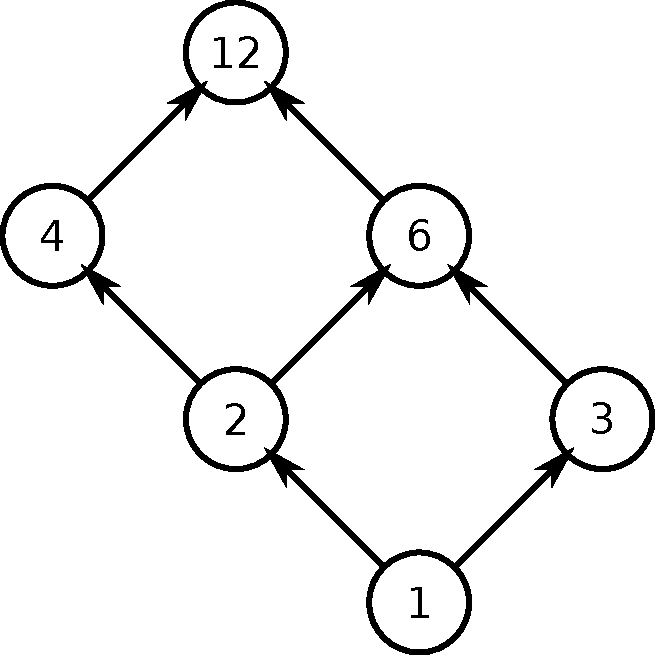
\includegraphics[scale=0.5]{Graphen/Primzahlen1.pdf}}
	\only<2|handout:2>{
\includegraphics[scale=0.5]{Graphen/Primzahlen2.pdf}}
	\only<3|handout:3>{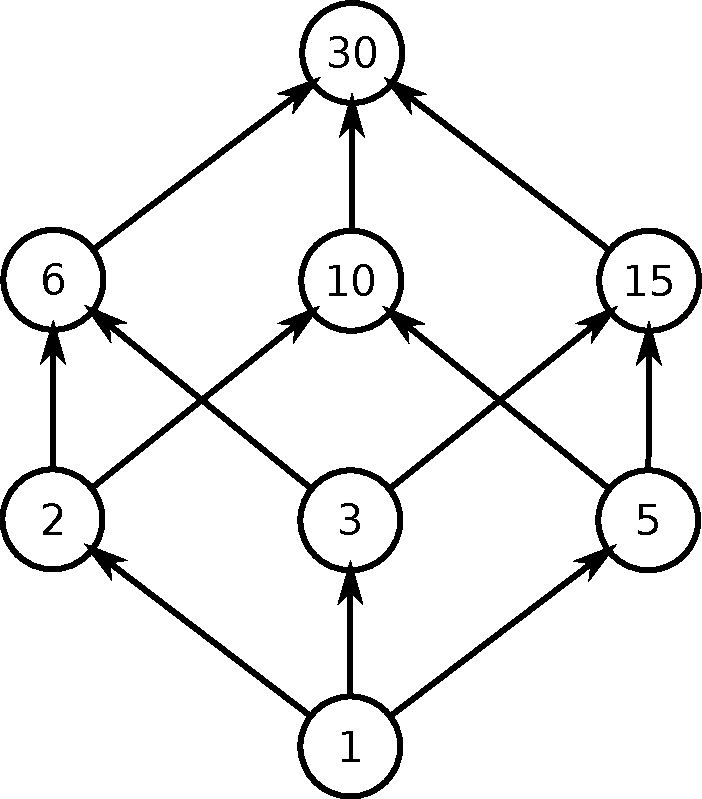
\includegraphics[scale=0.5]{Graphen/Primzahlen3.pdf}}
	\vfill
\end{frame}	

\begin{frame}{Lösung}
	\textit{Zeigen Sie: $$\forall n, m \in \N^+: n \text{ teilt } m \impl G_n \text{ ist Teilgraph von } G_m.$$}\\[2em] \pause
	Gelte also $n$ teilt $m$. Zu zeigen sind zwei Dinge:
	\begin{itemize}
		\item $V_n \subseteq V_m$
		\item $E_n \subseteq E_m \cap V_n \times V_n$
	\end{itemize}
	
\end{frame}

\begin{frame}{Lösung}
	\textit{Zuerst $V_n \subseteq V_m$.} \\[1em] \pause
	Sei $v \in V_n$ beliebig. Nach Definition gilt: $v$ teilt $n$. Da $n$ aber $m$ teilt, muss $v$ auch $m$ teilen, liegt also in $V_m$. Also gilt $$V_n \subseteq V_m$$ \pause
	
	\textit{Jetzt $E_n \subseteq E_m \cap V_n \times V_n$.} \\[1em] \pause
	Sei $p$ eine Kante mit $p = (x,y) \in E_n$. Wir haben gezeigt, dass dann $x,y \in V_m$ gilt. Außerdem gilt nach der Definition von $E_n$: $$x \text{ teilt } y \text{ und } y/x \text{ ist eine Primzahl}$$ Somit ist $p$ auch in $E_m$ und es gilt $$E_n \subseteq E_m$$.
\end{frame}

\section{Repräsentationen von Graphen}
\begin{frame}{Darstellung von Graphen}
	\begin{block}{Auf Papier}
		\begin{itemize}
			\item Graphische Darstellung
			\item Mengendarstellung
			\item Textuelle Beschreibung
		\end{itemize}
	\end{block}

	\pause
	\begin{block}{Im Rechner}
		Systematisches Abspeichern der Kanten notwendig.\\
		Knoten werden oftmals implizit verwendet.
		\begin{itemize}
			\item (Kantenliste)
			\item Adjazenzlisten
			\item Adjazenzmatrix
		\end{itemize}
	\end{block}
\end{frame}

\begin{frame}{Adjazenzlisten}
	\begin{Definition}
		In einer \emph{Adjazenzliste} werden zu einem Knoten $x$ alle Knoten eingetragen, die von $x$ aus direkt mit einer Kante verbunden sind.
	\end{Definition}

	\pause
	Für jeden Knoten existiert eine Liste, alle Listen werden meist in einem Feld gespeichert.
\end{frame}

\begin{frame}{Adjazenzlisten}
	\begin{Beispiel}
		\begin{columns}
			\column{0.4\linewidth}
			\begin{tikzpicture}[->,>=stealth,baseline=-5mm]
		        \matrix[matrix of math nodes,nodes={draw,circle,minimum size=5mm,inner sep=2pt},row sep=10mm,column sep=10mm,ampersand replacement=\&]
		        {
		          |(0)| 0 \& |(1)| 1 \& |(2)| 2 \\
		          \& |(3)| 3 \& \\
		        };
		        \draw  (0) -- (1);
		        \draw  (0) -- (3);
		        \draw  (2)  to [bend left] (3);
		        \draw  (2) -- (1);
		        \draw  (3) to [bend left] (2);
		        \draw  (0) to [bend left]  (2);
		        \path (2) edge [loop right] ();
		        \draw (1) -- (3);
	      	\end{tikzpicture}
			\column{0.4\linewidth}
				\pause
				Adjazenzlisten dazu:
				\begin{table}[H]
					\centering \vspace*{1em}
					\begin{tabular}{c|c} 0 & 1, 2, 3 \\ \hline 1 & 3 \\ \hline 2 & 1, 2, 3 \\ \hline 3 & 2 
					\end{tabular}  
				\end{table}
		\end{columns}
	\end{Beispiel}
\end{frame}

\begin{frame}{Adjazenzmatrix}
	\begin{Definition}
		Die \textbf{Adjazenzmatrix} eines Graphen $(V, E)$ mit $n$ Knoten ist die Matrix $A\in \{0,1\}^{n\times n}$ mit $$ A_{ij} = \begin{cases} 0 & (i,j) \notin E \\ 1 & (i,j) \in E \end{cases} $$ 
	\end{Definition}

	\medskip
	\emph{Achtung}: Bei dieser Definition müssen Matrix- und Knotenindizes mit dem gleichen Wert starten ($0$ oder $1$)
\end{frame}

\begin{frame}{Adjazenzmatrix}
\textbf{Adjazenzmatrix} \\
Verwende Matrix $A \in \{0, 1\}^{n \times n}$ \ mit \ $A_{ij} = 1 \gdw (i, j) \in E$

\bigskip
\begin{columns}
	\column{0.4\linewidth}
	\begin{tikzpicture}[->,>=stealth,baseline=-5mm]
	\matrix[matrix of math nodes,nodes={draw,circle,minimum size=5mm,inner sep=2pt},row sep=10mm,column sep=10mm,ampersand replacement=\&]
	{
		|(0)| 1 \& |(1)| 2 \& |(2)| 3 \\
		\& |(3)| 4 \& \\
	};
	\draw  (0) -- (1);
	\draw  (0) -- (3);
	\draw (1) -- (3);
	\draw  (2)  to [bend left] (3);
	\draw  (2) -- (1);
	\draw  (3) to [bend left] (2);
	\draw  (0) to [bend left]  (2);
	\path (2) edge [loop right] ();
	\end{tikzpicture}
	\column{0.4\linewidth}
	\[%
	A = \quad \kbordermatrix{%
		& \text{\llap{Nach \:}} 1 & 2 & 3 & 4 \\
		\text{\llap{Von \:}} 1 & 0 & 1 & 1 & 1 \\ 
		2 & 0 & 0 & 0 & 1 \\ 
		3 & 0 & 1 & 1 & 1 \\ 
		4 & 0 & 0 & 1 & 0
	}%
	\]
	%$$ A = \begin{pmatrix}  \end{pmatrix} $$
\end{columns}
	\pause
	\begin{block}{Besondere Eigenschaften der Adjazenzmatrix}
		\begin{itemize}
			\item Schlingen lassen sich an einer $1$ auf der Diagonalen erkennen (Wert von $A_{ii}$) 
			\item Bei ungerichteten Graphen ist $A$ immer symmetrisch (also $A_{ij} = A_{ji}$).
		\end{itemize}
	\end{block}
%	\begin{figure}[htp]
%		\centering
%		\includegraphics[width=\textwidth]{adjazenzmatrix}
%	\end{figure}
\end{frame}

\begin{frame}{Exkurs: Vergleich der Darstellungen}
	\begin{itemize}[<+->]
		\item Adjazenzliste: Speicherplatz abhängig von Anzahl der Kanten ($m$)\\
		Besser bei dünn besetzten Graphen. 
		\item Adjazenzmatrix: Immer gleich viel Speicherplatz ($n^2$)\\
		Besser bei dicht besetzten Graphen (kein Overhead für Listen nötig).
	\end{itemize}
\end{frame}


\begin{frame}{Exkurs: Vergleich der Darstellungen}
	% ACHTUNG: Leute hatten hier vllt. noch kein O-Kalkül in der VL, beware!
	\begin{itemize}[<+->]
		\item Adjazenzliste: Nachbarn ermitteln in $O(1)$\\
		Ermitteln ob $(i,j)$ adjazent sind in $O(n)$
		\item Adjazenzmatrix: Nachbarn ermitteln in $O(n)$\\
		Ermitteln ob $(i,j)$ adjazent sind in $O(1)$
	\end{itemize}

	\pause
	In der Praxis meistens (Varianten von) Adjazenzlisten verwendet.\\
	Denn: Die meisten Graphalgorithmen traversieren den Graphen, dafür sind Adjazenzlisten deutlich besser.
	
	\bigskip
	Viel mehr dazu in Algorithmen~I
\end{frame}


\begin{frame}	
	\begin{block}{Was ihr nun wissen solltet}
		\begin{itemize}
			\item Grundbegriffe der Graphen
			\item Zentrale Eigenschaften von Graphen
			\item Verschiedene Darstellungen von Graphen und deren Vorteile
		\end{itemize}
	\end{block}
	
	\begin{block}{Was nächstes Mal kommt}
		\begin{itemize}
			\item Graphen schön und gut - Aber jetzt wollen wir auch etwas damit machen!
			\item Warum dauert das so lange? - Laufzeitbetrachtungen
		\end{itemize}
	\end{block}
\end{frame}


\lastframe{0.65}{0}{xkcd/the_general_problem_974.png}{http://www.xkcd.com/974}
\slideThanks

\end{document}